
\documentclass{article} % For LaTeX2e
\usepackage{iclr2027_conference,times}

% Optional math commands from https://github.com/goodfeli/dlbook_notation.
\input{math_commands.tex}

\usepackage{hyperref}
\usepackage{url}
\usepackage{algorithm}
\usepackage{algorithmic}
\usepackage{amsmath}
\usepackage{amsfonts}
\usepackage{optidef}
\usepackage{dsfont}
\usepackage{booktabs}
\usepackage{xcolor}
\usepackage{wrapfig}



\title{EU-CRD: Managing Forecast Trust in Carbon-Aware Reinforcement Learning Scheduling via Epistemic Credit Redistribution}

% Authors must not appear in the submitted version. They should be hidden
% as long as the \iclrfinalcopy macro remains commented out below.
% Non-anonymous submissions will be rejected without review.

\author{Antiquus S.~Hippocampus, Natalia Cerebro \& Amelie P. Amygdale \thanks{ Use footnote for providing further information
about author (webpage, alternative address)---\emph{not} for acknowledging
funding agencies.  Funding acknowledgements go at the end of the paper.} \\
Department of Computer Science\\
Cranberry-Lemon University\\
Pittsburgh, PA 15213, USA \\
\texttt{\{hippo,brain,jen\}@cs.cranberry-lemon.edu} \\
\And
Ji Q. Ren \& Yevgeny LeNet \\
Department of Computational Neuroscience \\
University of the Witwatersrand \\
Joburg, South Africa \\
\texttt{\{robot,net\}@wits.ac.za} \\
\AND
Coauthor \\
Affiliation \\
Address \\
\texttt{email} }

% The \author macro works with any number of authors. There are two commands
% used to separate the names and addresses of multiple authors: \And and \AND.
%
% Using \And between authors leaves it to \LaTeX{} to determine where to break
% the lines. Using \AND forces a linebreak at that point. So, if \LaTeX{}
% puts 3 of 4 authors names on the first line, and the last on the second
% line, try using \AND instead of \And before the third author name.

% ---------------------------------------------------------------------
% RESULT MACROS. Every headline number that appears in more than one place
% lives here, so the post-campaign swap is one edit rather than a grep.
% Provenance for each is in reports/NUMBERS_MANIFEST.md.
% PLACEHOLDERS: still carry the pre-campaign (v4 build, pre-61043cf
% dispatcher) values. Do NOT submit until these are regenerated.
% ---------------------------------------------------------------------
% ---------------------------------------------------------------------
% FRAGILITY SWITCH. Whether the over-deferral failure mode exists at all is a
% result, not a premise, and the campaign may retire it. The definition is
% frozen in reports/APPF_PREREG.md: a checkpoint is fragile when training
% completion meets the contract, the same checkpoint meets it under stochastic
% clean decoding, and deterministic clean falls below 99.5%.
%
%   \FragileNonefalse + \FragilePatterntrue   >=2 fragile, both arms   (current)
%   \FragileNonefalse + \FragilePatternfalse  exactly 1, isolated case
%   \FragileNonetrue                          0, appendix deleted
% ---------------------------------------------------------------------
% \RiskSamplingtrue only if the retrained risk baselines are themselves evaluated
% under sampling. The old claim cannot be carried over from contaminated runs.
% \FragileUnresolvedtrue prints a visible [UNRESOLVED] tag next to every
% fragility claim. Currently OFF so the draft reads clean. The claim it
% guards is still ungraded, and the guard is now mechanical rather than
% visual: drl-manager/tests/test_appf_grading_done.py fails while the
% fragility claim renders and reports/APPF_GRADING.md does not exist.
\newif\ifFragileUnresolved \FragileUnresolvedfalse
\newcommand{\FragTag}{\ifFragileUnresolved\textcolor{red}{\,[UNRESOLVED]}\fi}
\newif\ifRiskSampling \RiskSamplingfalse
\newif\ifFragileNone   \FragileNonefalse
\newif\ifFragilePattern \FragilePatterntrue
\newcommand{\ResFragileCount}{one seed in four}
\newcommand{\ResFragileRange}{91 to 98\%}

\newcommand{\ResContain}{5\%}          % containment margin, EU-CRD vs matched Vanilla under Shuffle
\newcommand{\ResContainVan}{0.085}     % corruption increment, Vanilla   (Shuffle - Clean)
\newcommand{\ResContainEu}{0.063}      % corruption increment, EU-CRD
\newcommand{\ResContainDiD}{-0.022}    % difference in differences
\newcommand{\ResNoFcst}{0.196}         % No-Forecast PPO, clean
\newcommand{\ResVanShuffle}{0.269}    % Vanilla, shuffle
\newcommand{\ResVanClean}{0.184}      % Vanilla, clean   (also the ablation ladder's bottom rung)
\newcommand{\ResVanBlend}{0.184}      % Vanilla, blend
\newcommand{\ResEuShuffle}{0.255}      % EU-CRD, shuffle
\newcommand{\fix}{\marginpar{FIX}}
\newcommand{\new}{\marginpar{NEW}}

%\iclrfinalcopy % Uncomment for camera-ready version, but NOT for submission.
\begin{document}


\maketitle


\begin{abstract}
Carbon-aware datacenter schedulers increasingly rely on renewable energy forecasts, and deep reinforcement learning (DRL) schedulers now consume those forecasts directly in their observations. Trained on mostly accurate forecasts, a DRL policy learns to trust them unconditionally, and because standard training folds the forecast's contribution into a single return, it never learns to trust them only when warranted. When forecast quality degrades in deployment, that trust becomes a liability that standard training can neither isolate nor repair. This work proposes EU-CRD, a credit-assignment framework spanning training and deployment. During training, EU-CRD uses a counterfactual estimate of how much the forecast actually helped each decision and credits it for only that much. Because that estimate comes from a learned value model, EU-CRD trusts it only as far as a critic ensemble agrees on it, otherwise falling back on a forecast-free signal. A lightweight deployment-time auditor extends the same logic past training by monitoring the forecast against realized supply, adding no neural inference to the deployed policy. On a five-datacenter testbed with measured wind, conventional training's blind trust in a corrupted forecast leaves it worse off than using no forecast at all. The signal it was trained to exploit becomes a net liability. Against that penalty EU-CRD removes \ResContain{} of the carbon a coherent lie adds, at no measurable cost on clean forecasts, and keeps completion inside the service contract where conventional training does not. The separation appears under deterministic decoding, the form these schedulers are deployed in, and closes when actions are sampled.
\end{abstract}


\section{Introduction}
\label{sec:intro}

Training and serving large language models is reshaping datacentre workloads, and their electricity footprint grows with them \citep{jonesHowStopData2018}, while the largest cloud providers now report rising emissions even as they pledge carbon neutrality \citep{google2025EnvironmentalReport2025, microsoft2024EnvironmentalSustainability2024}. Integrating clean renewable energy sources (RES) is the primary countermeasure. However, renewable generation is intermittent. When and where green energy arrives determines when and where flexible tasks should run. A reactive scheduler can only reduce carbon against the supply it already observes, so the deferrable share of the load must be moved proactively towards green energy that has not yet arrived. Guided by a forecast, a scheduler can delay deferrable batch workloads into predicted green windows \citep{wiesnerLetsWaitAwhile2021} or route them towards datacentres about to receive green supply \citep{xuRenewableEnergyawareBig2018, zhangSustainableAIGCWorkload2023}. DRL has become the dominant way to learn both levers \citep{maoResourceManagementDeep2016, zhangGreenDRLManagingGreen2022}, and a learned policy consumes the forecast the way it consumes any other input, as part of its observation. Carbon-aware benchmarks have made that arrangement the default, building the carbon-intensity forecast into their reference agents' observations \citep{naug2024sustaindc, venkataswamyRARERenewableEnergy2022}. The forecast is therefore not an optional module attached to a scheduler but a channel the policy learns to rely on.

However, these forecast-based scheduling algorithms carry a hidden cost. Since the forecast is accurate for most of training, acting on it is rewarded far more often than it is punished, so the policy has every incentive to converge on unconditional trust. Standard training offers no corrective. The return rewards the decision and the forecast together and never isolates what the forecast contributed \citep{dietterich2018discovering}, so nothing in the gradient teaches the policy to tell a reliable forecast from an unreliable one. Worse still, systematic corruption never occurs during training at all, so conditional caution is never learned, and the unconditional trust is frozen into the policy that goes into service.

\begin{wrapfigure}{r}{0.35\textwidth}
\vspace{-\baselineskip}
\centering
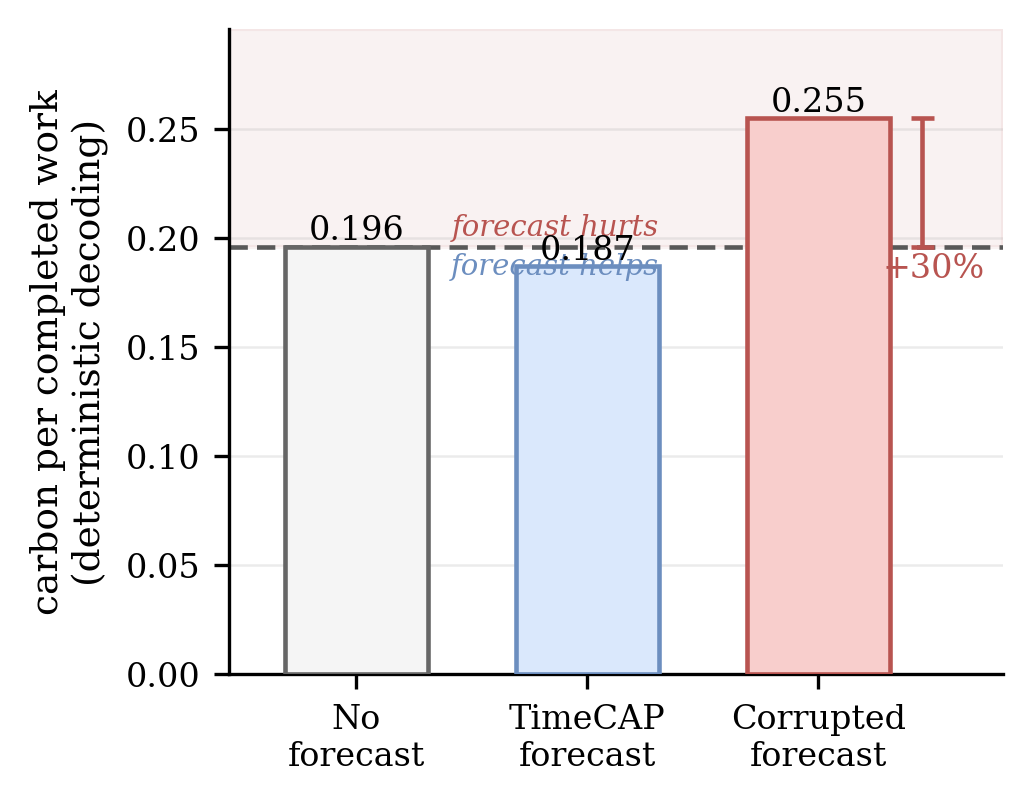
\includegraphics[width=\linewidth]{./figs/motivation.png}
\caption{The forecast as asset and liability. An accurate forecast lowers carbon below the no-forecast reference, a coherently reassigned one pushes it above.}
\label{fig:motivation}
\vspace{-0.5\baselineskip}
\end{wrapfigure}
Forecast quality is not stable over the lifetime of a deployed system. It degrades silently as sensors malfunction, models go stale and data pipelines fail \citep{polasekPredictingPhotovoltaicPower2023, meenalWeatherForecastingRenewable2022}. Adversarial work on load and solar forecasting shows the sharper form of this, where small perturbations of the weather inputs steer the output in arbitrary directions while the inputs still look like weather and the output still looks like a forecast \citep{chenExploitingVulnerabilitiesLoad2019, tangAdversarialAttacksSolar2021}. A plausible signal whose relationship to the realised supply has broken is the failure this work targets, in its mundane form rather than its adversarial one. A misconfigured site-to-feed mapping delivers one site's coherent forecast to another, and every value stays in range. Ordinary noise is not this failure. A policy trained on noisy forecasts has priced that noise into its returns, and the unconditional trust at issue here is what training on a mostly accurate signal produces rather than something noise can break. Such a forecast is no longer a noisy reference but a confident error. In Section~\ref{sec:experiments} a well-trained policy acts on it without hesitation, routing work toward datacentres it wrongly believes are about to turn green and emitting more carbon than a policy that ignores the forecast altogether (Figure~\ref{fig:motivation}). The forecast has become a liability.

Existing work does not target this failure. Risk-averse objectives \citep{2888116.2888133, di2012policy} and domain randomisation \citep{tobinDomainRandomizationTransferring2017} make the policy uniformly conservative regardless of forecast quality. The underlying issue is one of credit assignment. A policy gradient assigns a single advantage to each action, so the quality of the decision and the accuracy of the forecast are learned as one quantity, and a corrupted forecast keeps influencing every update. Counterfactual credit-assignment methods \citep{mesnard2020counterfactual, foersterCounterfactualMultiAgentPolicy2018} separate an action's contribution from factors beyond its control, but assume the exogenous signal is reliable, so they reproduce its corruption in the credit they assign. Uncertainty-aware methods \citep{korenUAMDPUncertaintyAwareMarkov2025} scale caution with confidence over the state, not over any single input channel. What this setting needs is credit attributed to the forecast channel at each transition, trusted only as far as it is reliable.

To close this gap, this work proposes EU-CRD (Epistemic-Uncertainty Counterfactual Responsibility Decomposition) for a hierarchical scheduler in which a global agent routes or defers each arriving workload and a local agent paces each datacentre's queue, so the forecast enters only through the global agent. During training, EU-CRD asks how each transition's outcome would have differed had the forecast matched reality, and splits the credit between the forecast and the routing decision. Because estimating the routing share relies on a learned value model that may itself be unreliable, EU-CRD gauges the epistemic uncertainty of that estimate from the disagreement of a critic ensemble and falls back on a model-free signal when the uncertainty is high. Transitions dominated by forecast responsibility are down-weighted, so corruption cannot reach the policy through the learning signal. A lightweight auditor applies the same test at deployment, monitoring the forecast against realised supply. Only the training signal and the input channel are touched, and at inference the policy is the plain backbone with no added latency. Our contributions are summarised as follows.
\begin{itemize}
\setlength{\itemsep}{0pt}\setlength{\topsep}{2pt}\setlength{\parskip}{0pt}
\item \textbf{Counterfactual responsibility decomposition.} This work proposes EU-CRD, a credit-assignment framework that attributes responsibility transition by transition and quarantines the learning signal a corrupted forecast injects, while retaining the forecast's value on clean inputs. To our knowledge, it is the first to handle forecast corruption at the credit-assignment level, treating the forecast as a single corruptible channel rather than defending the observation wholesale.
\item \textbf{Epistemic-uncertainty gating.} A soft gate scores each counterfactual estimate by critic-ensemble disagreement and falls back on a model-free signal when the estimate cannot be trusted, so the decomposition is used only as far as it is sound.
\item \textbf{Evaluation under forecast corruption.} On a five-datacenter testbed driven by measured wind, a corrupted forecast pushes conventional training past the carbon of using no forecast at all. EU-CRD removes \ResContain{} of that penalty while matching conventional training on clean forecasts, and is the only compared method that both consumes the forecast and keeps completion inside the service contract when it turns hostile. This advantage is specific to deterministic decoding and does not survive sampled actions (Section~\ref{sec:main}).
\end{itemize}


\section{Related Work}
\label{sec:related}
\subsection{Carbon-aware and renewable-driven scheduling}
Carbon-aware scheduling matches demand to low-carbon supply, spatially by routing to cleaner sites and temporally by deferring tolerant jobs to greener windows. One line is heuristic or combinatorial. \citet{wiesnerLetsWaitAwhile2021} shift load by a forecast-driven threshold-deferral rule, and \citet{schweisgutCarbonAwareWorkflowScheduling2025} solve carbon-aware workflow scheduling as a combinatorial optimisation under a deadline constraint. Recent work learns these decisions with RL. \citet{jayanettiMultiAgentDeepReinforcement2024} use a multi-agent actor-critic across datacentres, \citet{alqithamiEcoFairCHMARLScalableConstrained2025a} add a primal-dual emission-budget layer over PPO, and \citet{gaoSelfAttentionMechanismsHPC2025} schedule HPC jobs with a gated-transformer PPO close to the backbone used here. \citet{yuCarbonEfficientDataCenter2025} model forecast error explicitly rather than assuming a point prediction. These systems differ in whether and how well they exploit a forecast, not in how safely they consume one, and even where forecast error is modelled it is treated as benign noise.

\subsection{Credit assignment and exogenous-signal decomposition}
Credit assignment isolates an action's true influence on future return. A counterfactual line marginalises out a single agent action via a centralised critic \citep{foersterCounterfactualMultiAgentPolicy2018}, strips exogenous variance with future-conditional hindsight baselines \citep{mesnard2020counterfactual, harutyunyanHindsightCreditAssignment2019}, or assigns Shapley-value credit \citep{liShapleyCounterfactualCredits2021}. Closest to this work, \citet{dietterich2018discovering} remove the exogenous state variables and rewards an action cannot influence, leaving a lower-variance endogenous MDP, and \citet{efroni2022sample} formalise the exogenous-information MDP. Removal makes these methods immune to corruption of the exogenous signal, but discards whatever value the signal carried. Decision-focused learning approaches the interface from the opposite side, training the predictor under the downstream decision loss \citep{elmachtoub2022smart, wilder2019melding}. This work instead keeps the predictor frozen and changes how the policy assigns credit to its output. The counterfactual line trusts the signal it conditions on, and the exogenous-MDP line escapes corruption only by giving the signal up. Neither retains a corruptible signal's value conditionally, and neither gates credit by confidence in the decomposition itself.

\subsection{Risk-sensitive, uncertainty-aware, and input-robust RL}
A standard route to robustness makes the policy risk-sensitive or uncertainty-aware. The risk-sensitive family reshapes the objective, optimising conditional value-at-risk \citep{2888116.2888133} or penalising return variance \citep{di2012policy}, with distributional and utility-based variants \citep{pmlr-v80-dabney18a}. Domain randomisation \citep{tobinDomainRandomizationTransferring2017} perturbs training inputs instead. Both make the policy uniformly conservative, sacrificing clean-forecast performance whether or not the signal is degraded. A second family estimates model confidence over the state. \citet{anCLUESafeModelBased2023} read epistemic uncertainty from an ensemble to stay conservative on unfamiliar states during energy control, and \citet{korenUAMDPUncertaintyAwareMarkov2025} run risk-constrained RL directly on a probabilistic forecast. Confidence over the state, however, is not confidence in any single input channel. A third family defends the observation itself, through smoothness regularisation \citep{zhang2020robust}, training against a learned adversary \citep{zhang2021robust}, or denoising before the policy acts \citep{yang2024dmbp}. These desensitise or repair every dimension at once, without identifying which decisions the corruption affected, and cover only perturbations representable at training time. Two simpler alternatives deserve mention. Dropping the forecast during training is the training-time analogue of what this work does through credit, at the cost of uniform rather than selective caution, and an explicit forecast-confidence input needs that confidence to be trustworthy exactly when the forecast is not. EU-CRD instead acts on the learning signal, down-weighting only the channel that is corrupted.

\section{Methodology}
\label{sec:method}
\subsection{Problem Formulation}
\label{sec:problem}

An online stream of deferrable jobs, each with a compute size and a deadline $d_j$, is scheduled across $N$ geo-distributed datacentres. A DC $i$ may draw on on-site wind supplying green power $g_i(t)\ge 0$, zero at sites without it, with any shortfall met by the grid. Since grid power is far more carbon-intensive ($\kappa^{\text{green}}_i \ll \kappa^{\text{brown}}_i$), emissions come almost entirely from this shortfall.

Control is hierarchical and learned with RL. At a fixed control interval a global router $\pi_G$ routes or defers the batch of jobs that arrived since the last interval, conditioned on per-DC state and a green-power forecast $\hat{\mathbf{y}}_i=(\hat{y}^{\,s}_i,\hat{y}^{\,l}_i)$ over a short and a long horizon. A local scheduler $\pi_L$ then paces each DC's queue from its own partial view (Section~\ref{sec:mdp}). The forecast enters only through $\pi_G$, since only the route-or-defer decision converts its information into carbon savings, and the responsibility decomposition later anchors there. The joint policy $\pi_\theta=(\pi_G,\pi_L)$ is trained with PPO to maximise $J(\theta)=\mathbb{E}_{\pi_\theta}[\sum_t \gamma^t r_t]$, serving the operational goal of minimising carbon subject to an SLA on timely completion,
\begin{equation}
\min_{\theta}\ \mathbb{E}\!\left[\sum_{t,i}\kappa^{\mathrm{brown}}_i b_i(t)+\kappa^{\mathrm{green}}_i\big(u_i(t)-b_i(t)\big)\right]\quad\text{s.t.}\quad\frac{1}{|\mathcal{J}|}\sum_{j}\mathds{1}\!\left[f_j\le d_j\right]\ge\tau ,
\label{eq:objective}
\end{equation}
\begin{wrapfigure}{r}{0.28\textwidth}
\vspace{-0.6\baselineskip}
\centering
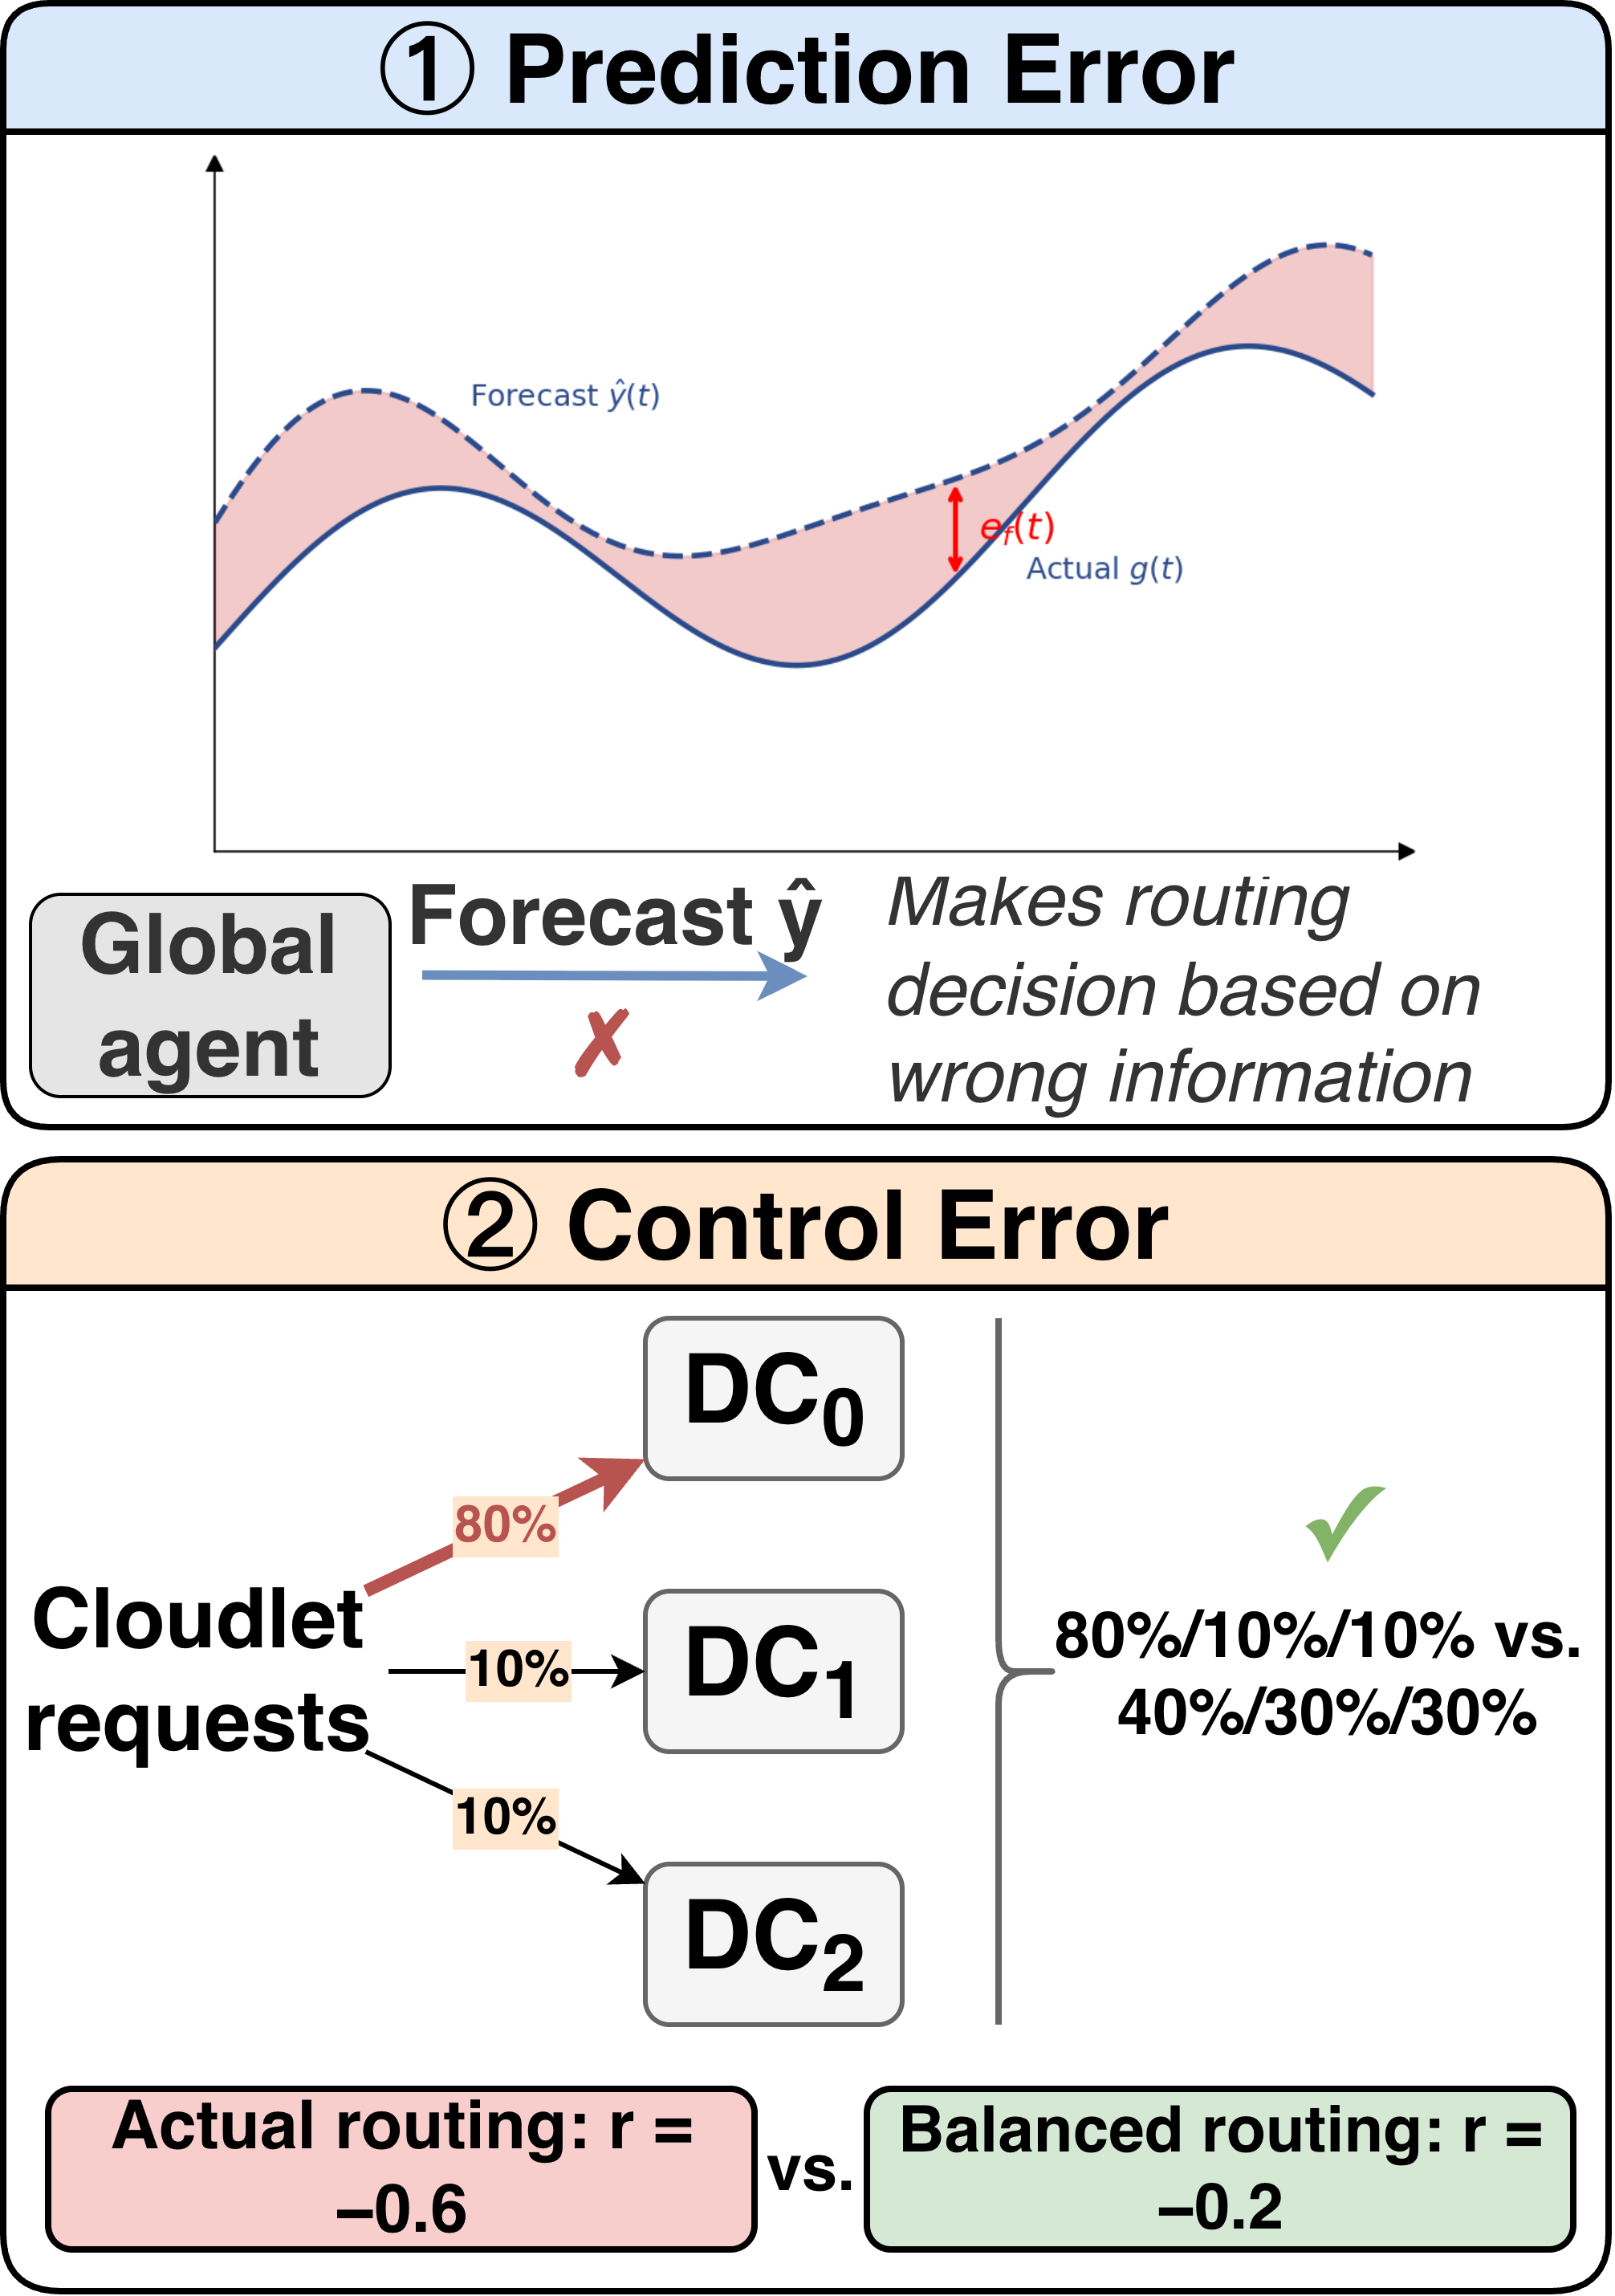
\includegraphics[width=\linewidth]{./figs/fig1_concept_stacked.png}
\caption{Standard training charges the policy for both the prediction error (top) and the control error (bottom).}
\label{fig:concept}
\vspace{-0.4\baselineskip}
\end{wrapfigure}
where $u_i(t)$ is the total power demand at DC $i$, $b_i(t)=\max\{0,\,u_i(t)-g_i(t)\}$ the brown power drawn once on-site green is exhausted, $\kappa^{\text{green}}_i$ the small embodied intensity of on-site generation (values in Section~\ref{sec:experiments}), $\mathcal{J}$ the job set, $f_j$ the completion time of job $j$, and $\tau$ the required completion rate. The reward scalarises this objective at the action level, charging each routing decision its marginal carbon and crediting expected timely completion, with an overdue-deferral backstop guarding deadlines. The constraint is handled approximately rather than enforced, so completion is reported alongside carbon as an independent axis throughout Section~\ref{sec:experiments}.

The difficulty this work targets is that $g_i(t)$ is exogenous and the router acts on its forecast, not its realisation. The return therefore mixes a control error, acting poorly given correct information, with a prediction error $e_i(t)=\hat{y}^{\,s}_i(t)-g_i(t)$ (Figure~\ref{fig:concept}). The error is anchored on the short horizon because that is the component the router consumes when committing a batch, and a corrupted long horizon reaches the policy through the same channel as the predicted window draws near.  Standard policy-gradient credit assigns the whole advantage to the acting policy. The harm is not merely the added gradient variance studied in exogenous-decomposition work. Because the forecast is mostly accurate during training, transitions whose return the forecast supplied are almost always rewarded, and the policy learns to trust the signal unconditionally. That learned dependence is precisely what a corrupted forecast exploits at deployment. What Eq.~\ref{eq:objective} leaves open is therefore a credit scheme that attributes each transition's advantage to its source, the forecaster or the acting policy, and updates the policy only on the controllable share. Down-weighting forecast-dominated transitions weakens that dependence and preserves reactive competence that survives when the forecast degrades.

This work proposes EU-CRD, illustrated in Figure~\ref{fig:framework-full}. During training a counterfactual decomposition attributes each transition to the forecaster or to the routing policy and updates the policy only on the share it controls, and after deployment an auditor tracks whether the forecast still matches reality. The rest of this section develops these components in turn.

\begin{figure*}[t]
    \centering
    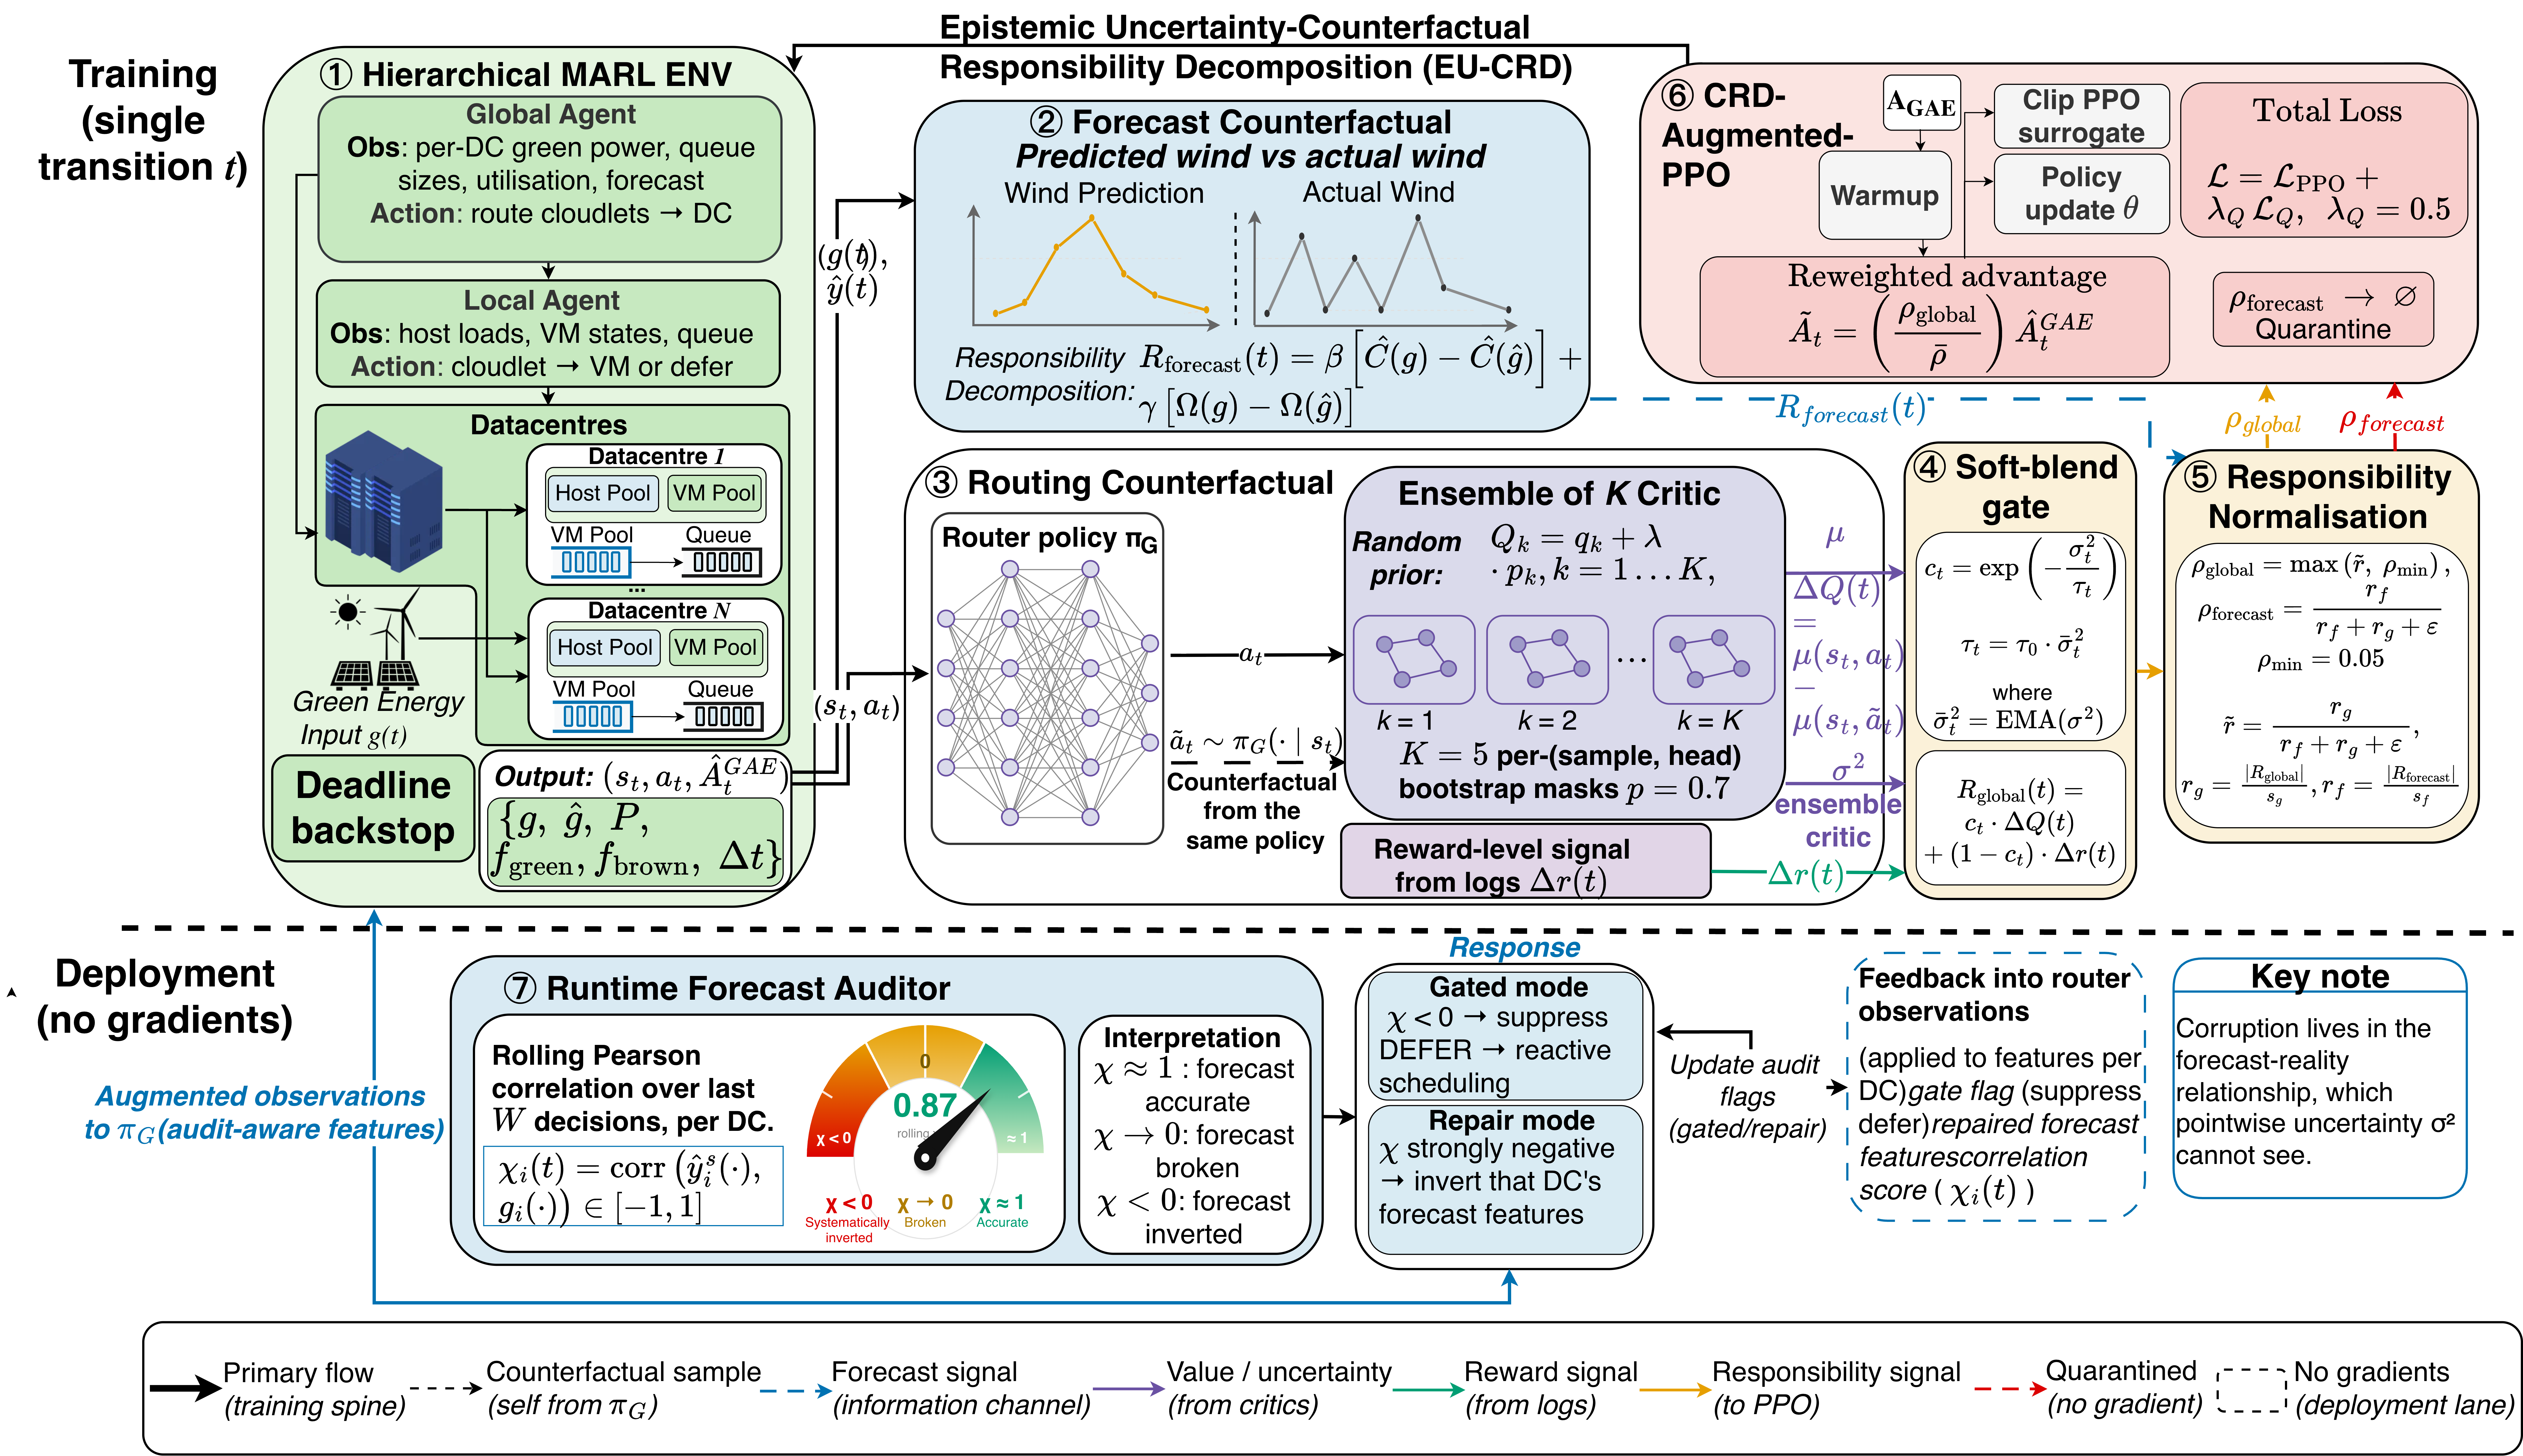
\includegraphics[width=1.0\linewidth]{./figs/new_EUCRD_drawio_nature.png}
    \caption{The EU-CRD training loop: forecast, decision, outcome, counterfactual, responsibility, gated credit, policy update. The decomposition splits each transition's credit between the forecast and the routing action, ensemble disagreement $\sigma^2$ gates how far the value-based estimate is trusted over the model-free fallback, and the weights rescale the PPO advantages. Only the auditor stays active at deployment.}
    \label{fig:framework-full}
    \vspace{-12pt}
\end{figure*}

\subsection{Hierarchical MDP Design}
\label{sec:mdp}
The global router acts once per control interval on the waiting batch, observing per-DC green power, queue length and utilisation, the forecast features $\hat{\mathbf{y}}_i$ (short- and long-horizon mean, trend, and time-to-peak), and per-job size and deadline. Its action routes each of up to $B$ jobs to one of the $N$ DCs or to a DEFER slot, a factored space $\{0,\dots,N\}^{B}$ treated as $B$ per-job decisions rather than one joint distribution ($B{=}128$ in Section~\ref{sec:experiments}). A deadline backstop shared by all methods force-routes any job whose deadline is imminent, bounding how long a job can be held. Each DC's local scheduler, its parameters shared across sites so one policy serves any number of DCs, observes its own hosts, VMs, and queue, and its action is a release count $k\in\{0,\dots,K\}$ that paces how fast the queue drains. The local agent never observes the forecast. Full observation and action specifications are in Appendix~\ref{app:testbed}.

The two reward channels mirror this division. The global reward $r^{G}_t$ carries the carbon objective through a per-job marginal-carbon term, a congestion term $\hat{P}_i$ estimating the probability that a job routed to DC $i$ still finishes on time, and a deferral cost priced by an urgency ramp as the job's slack runs out. The local reward $r^{L}_t$ is a standard, forecast-independent quality-of-service signal (completions, mean wait, VM-utilisation imbalance, backlog, invalid actions). Carbon and the forecast enter only through $r^{G}_t$. Full definitions and coefficients are in Appendix~\ref{app:reward}. The decomposition of the next subsection dissects the credit carried by $r^{G}_t$ alone. The local channel passes through untouched.

\subsection{Counterfactual Responsibility Decomposition}
\label{sec:crd}

EU-CRD attributes each transition's outcome, the step carbon and wasted green power plus the downstream return, to the two sources that shape it, the forecaster supplying the information and the global router acting on it. The local scheduler carries no confound and trains conventionally.

Responsibility is measured counterfactually. Replace the source with a fixed reference, hold everything else equal, and record how much the outcome changes (Fig.~\ref{fig:framework-full}). The forecast probe replaces the forecast by the realisation while the global routing stays fixed. The routing probe replaces the router action by a reference action drawn from the router's own current policy while the information stays fixed. Each probe yields a per-transition responsibility signal $R_k(t)$ with $k\in\{\text{forecast},\text{global}\}$. Eq.~\ref{eq:rho} normalises these signals into responsibility weights $\rho_k(t)$, which reweight the policy update, quarantining the forecaster share and rescaling the advantage of the router.

For the forecaster, the reference is the realisation itself. Let $g(t)$ denote the realised per-DC green power at step $t$ and $\hat{g}(t)$ the predicted green-power profile carried by the forecast $\hat{\mathbf{y}}$. With the realised power demand held fixed, the step carbon $\hat{C}(\cdot)$ and the green-waste ratio $\Omega(\cdot)$ are evaluated under both profiles. Writing $\Delta\hat{C}(t)=\hat{C}(g(t))-\hat{C}(\hat{g}(t))$ and $\Delta\Omega(t)=\Omega(g(t))-\Omega(\hat{g}(t))$, the two gaps are combined with fixed weights $\beta{=}0.5$, $\gamma{=}0.3$ (identical across methods) into
\begin{equation}
R_{\text{forecast}}(t)=\beta\left|\frac{\Delta\hat{C}(t)}{C_{\max}(t)}\right|
+\gamma\big|\Delta\Omega(t)\big|,
\label{eq:rfcst}
\end{equation}
which measures the outcome gap between the forecast promised and what arrived. Two details of this form are load-bearing. The carbon gap is divided by $C_{\max}(t)$, the step's all-brown carbon, because the raw gap is a timestep-scaled quantity in kilograms while the waste gap is a dimensionless ratio. Without the normalisation the two terms differ by orders of magnitude and $\beta$ and $\gamma$ do not weight what they appear to weight. The terms enter as magnitudes because they carry opposite signs for the same forecast error and would partially cancel, so a signed sum passes through zero at the cancellation point and under-attributes a genuinely large error. The attribution pipeline consumes $|R_{\text{forecast}}|$ in any case. Because both profiles are evaluated under the realised placement, errors at datacentres carrying no load contribute nothing. The signal is large only where wrong information met actual work. For the router, the reference action $\tilde{a}_t$ is drawn from the router's own policy at the same state, a COMA-style counterfactual baseline that holds the information fixed and varies only the action. The routing responsibility is the value gap between the chosen action $a_t$ and this reference action $\tilde{a}_t$,
\begin{equation}
R_{\text{global}}(t)=Q^{\pi}\!\big(s_t,a_t\big)-Q^{\pi}\!\big(s_t,\tilde{a}_t\big),
\label{eq:rglobal}
\end{equation}
the part of the outcome attributable to the specific action the router chose, relative to a typical action from its own policy given identical information. Drawing the reference from the policy itself keeps the gap centred, so ordinary routing incurs no systematic charge. Unlike Eq.~\ref{eq:rfcst}, this gap has no closed form, since $Q^{\pi}$ is not available and must be estimated from learned value functions. The estimator and its calibration are the subject of the epistemic-uncertainty component presented in the next subsection.

The two signals are normalised into per-transition responsibility weights
\begin{equation}
\rho_k(t)=\max\!\left(\frac{|R_k(t)|\,/\,s_k(t)}{\sum_{k'}|R_{k'}(t)|\,/\,s_{k'}(t)+\varepsilon},\;
\rho_{\min}\right),
\label{eq:rho}
\end{equation}
where $\varepsilon{=}10^{-8}$ prevents division by zero and $\rho_{\min}$ is a floor no share may fall below. Two stages precede the ratio. First, an anomaly gate keeps only the excess of the forecast signal over its own recent behaviour,
\begin{equation}
R^{+}_{\text{forecast}}(t)=\max\!\big(|R_{\text{forecast}}(t)|-(\mu_f+z\,\sigma_f),\;0\big),
\label{eq:anom}
\end{equation}
with $\mu_f$ and $\sigma_f$ running estimates of the mean and standard deviation of $|R_{\text{forecast}}|$. Ordinary residual error exists in every regime, and charging it would suppress learning precisely on the informative wind-ramp transitions. Only anomalous error is quarantined. The gate acts on the raw signal, before any rescaling, so that a sustained corruption cannot be absorbed into the running scale and rendered invisible. Second, each signal is divided by $s_k(t)$, a running estimate of its own typical magnitude, so the shares compare relative anomaly rather than native units. The ratios sum to one before the floor is applied and only approximately after it, since the floor acts on each share independently. Only $\rho_{\text{global}}$ enters the update, and it is renormalised by its batch mean, so the reweighting does not depend on the pair summing exactly to one. The rescaling is necessary because the two signals are incommensurate. $R_{\text{global}}$ grows with the critic's scale while $R_{\text{forecast}}$ stays in reward-proxy units, so raw ratios would pin the routing share near one. Dividing by each running scale is what makes the shares comparable at all. It is the anomaly gate of Eq.~\ref{eq:anom}, not the rescaling, that restricts the charge to anomalous error. Together they leave the router's share untouched under ordinary residual error and shift credit onto the forecaster only when its error grows large relative to its own recent history. The forecaster share $\rho_{\text{forecast}}$ is then quarantined from the policy gradient while the router advantage is rescaled by $\rho_{\text{global}}$, divided by the batch mean share so that the average responsibility multiplier is one. The policy is not punished for reasonable decisions taken on misleading forecasts, so trust in the forecast is preserved during training and managed at deployment instead. Two properties are stated plainly. Eq.~\ref{eq:rfcst} holds the router's actions fixed, making it a local responsibility proxy rather than the full causal effect of a correct forecast, and $R_{\text{forecast}}$ is per-step while $R_{\text{global}}$ carries downstream return, so Eq.~\ref{eq:rho} aligns magnitudes but not horizons. Both bias the decomposition towards under-quarantining. In causal terms, Eq.~\ref{eq:rfcst} is a controlled direct effect. It coincides with the forecast-induced outcome error exactly when the outcome depends on the forecast only through the two evaluated supply profiles, with the placement held at its realised value. The action-mediated remainder, whatever a different routing response to the corrupted signal would have added, stays in the router's account by construction, so the quarantined share errs low rather than high.

\subsection{Epistemic Uncertainty and Soft Blending}

The routing responsibility (Eq.~\ref{eq:rglobal}) needs $Q^{\pi}$, which has no closed form and must be estimated from a learned critic. That estimate is unreliable early in training, on rarely visited states, and on the out-of-distribution states a corrupted forecast drives the agent into. Its reliability at each transition is a question of epistemic uncertainty.

We estimate it with an ensemble of $K$ critics $\{Q_{\theta_k}\}_{k=1}^{K}$, trained on bootstrapped targets with randomised prior functions to keep the members diverse \citep{osband2016deep, osband2018randomized}. Their mean gives the value gap $\Delta Q(t)=\mu(s_t,a_t)-\mu(s_t,\tilde{a}_t)$ with $\mu(s,a)=\tfrac{1}{K}\sum_{k} Q_{\theta_k}(s,a)$, Uncertainty is taken as $\sigma^2_t=\operatorname{Var}_{k} Q_{\theta_k}(s_t,a_t)+\operatorname{Var}_{k} Q_{\theta_k}(s_t,\tilde{a}_t)$, small on familiar states and large on undertrained ones. This upper-bounds the variance of the difference whenever the two estimates are positively correlated, so the gate is deliberately conservative. The member-wise alternative $\operatorname{Var}_{k}\!\big[Q_{\theta_k}(s_t,a_t)-Q_{\theta_k}(s_t,\tilde{a}_t)\big]$ would discount correlated errors that cancel in the difference. The summed form is kept because an overestimated $\sigma^2$ only pushes the gate towards the model-free fallback, the failure-safe direction.

$\Delta Q$ is paired with a coarser reward-level signal $\Delta r(t)$ computed analytically from the decision-time state rather than from a learned value function. Each routed job is scored by the green fit of the datacentre it is sent to, and the reference action is scored the same way,
\begin{equation}
\Delta r(t)=\alpha\,\operatorname{mean}_{j}\big[g_t(a_{t,j})-g_t(\tilde{a}_{t,j})\big],
\qquad g_t(\textsc{defer})=0 ,
\label{eq:deltar}
\end{equation}
where $g_t(i)$ is the green ratio observed at datacentre $i$ at the moment of the decision, the same per-DC quantity the router sees in its observation. Deferral slots score zero because immediate green fit is undefined for a job that is not placed. The long-horizon value of deferring is the $\Delta Q$ path's responsibility. $\Delta r$ therefore ignores long-horizon effects, and in exchange uses no learned value function, so unfamiliar states cannot corrupt it. Aligning it with the carbon objective matters. A load-balance proxy would track a quantity the reward does not contain and can disagree with $\Delta Q$ in sign. A soft blend of the two gives the routing responsibility,
\begin{equation}
R_{\text{global}}(t)=c_t\,\Delta Q(t)+(1-c_t)\,\Delta r(t),
\qquad
c_t=\exp\!\big(-\sigma^2_t/\tau_t\big),
\qquad
\tau_t=\tau_0\,\bar{\sigma}^2_t ,
\label{eq:blend}
\end{equation}
where $\sigma^2_t$ is the ensemble disagreement at the transition and $\bar{\sigma}^2_t$ an exponential moving average of it over recent batches. As $\sigma^2_t\!\to\!0$ the gate $c_t\!\to\!1$ and the credit follows $\Delta Q$, while large disagreement drives $c_t\!\to\!0$ and the credit falls back on $\Delta r$. Scaling the temperature by the running level of disagreement makes the gate scale-free. A transition whose disagreement is $m$ times the prevailing level receives $c_t=\exp(-m/\tau_0)$ irrespective of the absolute magnitude of $\sigma^2$, so a single $\tau_0$ calibrates the gate throughout training. This blended $R_{\text{global}}(t)$ is the routing responsibility that the decomposition normalises in Eq.~\ref{eq:rho}.

Rather than being trusted unconditionally, the value-based credit is thus calibrated by the ensemble's confidence in it. Its contribution is isolated in the Section~\ref{sec:experiments} ablation, which fixes $c_t\equiv1$.



\subsection{CRD-Augmented Policy Optimisation}
\label{sec:crd-ppo}

The responsibility weights act on learning through the advantage. The router optimises the clipped PPO surrogate on a reweighted advantage,
\begin{equation}
\tilde{A}_t = \frac{\rho_{\text{global}}(t)}{\bar{\rho}}\,\hat{A}_t,
\label{eq:reweight}
\end{equation}
where $\hat{A}_t$ is the GAE advantage, $\rho_{\text{global}}$ the routing share from Eq.~\ref{eq:rho}, and $\bar{\rho}$ its batch mean. The policy gradient then carries only the fraction of the outcome attributable to the routing decision. The local scheduler carries no responsibility term and is optimised by standard PPO.

Dividing by the batch mean $\bar{\rho}$ normalises the mean responsibility multiplier to one, avoiding the systematic first-order reduction in update scale that plain multiplication by $\rho_{\text{global}}\le1$ would cause. It does not preserve the mean advantage exactly, since $\rho_{\text{global}}$ and $\hat{A}$ may be correlated.

The ensemble critic that produces $\Delta Q$ and $\sigma^2$ is trained jointly. Its $K$ heads follow a bootstrapped temporal-difference loss $\mathcal{L}_Q$, added to the surrogate with a coefficient $\lambda_Q$ to give the total objective $\mathcal{L}=\mathcal{L}_{\text{PPO}}+\lambda_Q\mathcal{L}_Q$. The separate value head keeps learning the unbiased return, so quarantining the forecaster share never biases the bootstrap targets.

Three stabilisers keep the reweighting from destabilising the policy. The responsibility signals are detached, so they scale the advantage as constants. Reweighting waits out a warmup until the ensemble critic is competent. The floor $\rho_{\min}$ guarantees the router a minimal share even when the forecaster dominates. The decomposition adds a small set of constants, namely the running-scale EMA rate, the anomaly-gate threshold $z$ and its decay, the gate temperature $\tau_0$ and its EMA rate, the floor $\rho_{\min}$, the $\Delta r$ coefficient $\alpha$, and the warmup length. A single setting, listed in Appendix~\ref{app:training}, is used for every method, condition and seed, and none was tuned per corruption.

Algorithm~\ref{alg:eucrd} (Appendix~\ref{app:algorithm}) summarises the full training arm. Training thus preserves the forecast's value where it earns trust while removing the unconditional reliance standard training instils. A forecast that degrades after deployment falls to the runtime auditor.

\subsection{Runtime Forecast Auditor}
\label{sec:auditor}
The training arm preserves trust in the forecast, which is safe only while the forecast stays accurate. A lightweight deployment-time check therefore accompanies the policy. For each DC, a rolling Pearson correlation $\chi_i$ between the short-horizon forecast and the realised green power flags a forecaster that has decoupled from reality, gating deferral once averaged trust collapses and inverting a DC's features under strong negative correlation. Correlation rather than the training-time $\sigma^2$ is the right statistic here. A plausible forecast that happens to lie is not an unfamiliar state, and the corruption lives in the forecast--outcome relationship that $\chi_i$ measures directly. The auditor needs no training and leaves the policy untouched, so it retrofits without retraining. Under an inverted forecast the auditor restores a corrupted policy to its clean operating point on both carbon and completion, with thresholds, window, and the full evaluation in Appendix~\ref{app:auditor}.

\section{Experiments}

\label{sec:experiments}
\subsection{Experiment Setup}
\label{sec:setup}
The testbed is a five-datacentre environment on CloudSim Plus \citep{silvafilhoCloudSimCloudComputing2017}, three low-carbon sites carrying SDWPF 2021 wind \citep{zhouSDWPFDatasetSpatial2024} at staggered time-zone offsets, and a workload of 8000 deferrable jobs with per-job deadlines. Only the global policy sees the forecast, from a TimeCAP forecaster \citep{ren2026timecap}, and both policies use PPO \citep{schulman2017proximal} on a GTrXL backbone \citep{parisotto2020stabilizing}. Grid intensities, fleet sizes and the full configuration are in Appendix~\ref{app:testbed}. Under the deterministic decode reported throughout, the forecast lowers carbon by 5\% against an identical policy trained without it (14\% under sampling, Appendix~\ref{app:stoch}), and the asymmetry that motivates this work is already visible. A clean forecast is worth 5\% while a corrupted one costs Vanilla 36\% of its own clean carbon. The comparison set is Vanilla PPO and four risk-sensitive objectives, CVaR \citep{2888116.2888133}, mean-variance \citep{di2012policy}, risk-sensitive utility \citep{6855488} and a distributional CVaR variant, all sharing the architecture, environment and budget. Vanilla PPO and EU-CRD use four seeds, the single-seed baselines are indicative, and hyperparameters are in Appendix~\ref{app:training}. Carbon per completed work can be gamed, since abandoning jobs runnable only in carbon-intensive windows lowers the reported carbon on the remainder. It is therefore compared only at matched completion ($\geq 99.5\%$) with checkpoints selected on clean-forecast validation, never across decodes, while under corruption completion is itself an outcome and both metrics are reported jointly. Corruption is injected at evaluation only, and the two operators play different roles. Shuffle reassigns forecasts across datacentres, so each site receives another site's coherent and internally consistent prediction. That is the failure of Section~\ref{sec:intro}. The signal stays plausible while its relationship to the realised supply breaks, and its real-world cause is a misconfigured site-to-feed mapping. Blend replaces the forecast with uninformative constants, which removes information without misdirecting it. Blend is therefore a control rather than a second instance of the target failure, and the pair separates the harm of losing the signal from the harm of being lied to by it. The primary carbon endpoint is Shuffle.

\subsection{Main Comparison}
\label{sec:main}

\begin{table}[t]
\caption{Carbon per completed work, completion rate in parentheses (\%), under forecast corruption at deterministic decoding. Medians over iso-eligible seeds. The checkpoint rule and seed counts are in Section~\ref{sec:setup}, per-seed values in Appendix~\ref{app:perseed}. $\Delta_{\text{corr}}$ is the absolute carbon a coherent lie adds, Shuffle minus Clean of the tabled medians, so a method is not rewarded for being poor on clean forecasts the way a Shuffle/Clean ratio would be. C$_{\min}$ is the lowest completion over the iso-eligible seeds and all conditions. Each arm's decode-fragility seed is excluded by the same rule (Appendix~\ref{app:failure}). $\dagger$: completion below 99.5\%, carbon deflated by dropped work and not highlighted. Dashes mark undefined cells. Vanilla PPO is both the standard-training reference and the complete ablation of the method. It differs from EU-CRD in one configuration key, so the comparison is matched by construction rather than by argument (Appendix~\ref{app:ablation}).}
\label{tab:main}
\centering
\small
\begin{tabular*}{\linewidth}{@{\extracolsep{\fill}}lccccc@{}}
\toprule
Method & Clean & Blend & Shuffle & $\Delta_{\text{corr}}$ & C$_{\min}$ \\
\midrule
\multicolumn{6}{@{}l}{\textit{Reference point}} \\
No-Forecast PPO   & 0.196\,(99.7) & -- & -- & -- & 99.7 \\
\multicolumn{6}{@{}l}{\textit{Standard training}} \\
Vanilla PPO       & \textbf{0.184}\,(99.7) & \textbf{0.184}\,(100) & 0.269\,(100) & $+0.085$ & 95.6 \\
\multicolumn{6}{@{}l}{\textit{Robust training}} \\
CVaR-PPO          & 0.138$^\dagger$(93.5) & 0.102$^\dagger$(97.7) & 0.051$^\dagger$(48.1) & -- & 48.1 \\
Mean-variance     & 0.179$^\dagger$(30.6) & 0.154$^\dagger$(18.0) & 0.154$^\dagger$(18.0) & -- & 18.0 \\
Risk-sensitive    & 0.116$^\dagger$(50.1) & 0.143$^\dagger$(19.8) & 0.177$^\dagger$(19.2) & -- & 19.2 \\
Dist-CVaR         & 0.130$^\dagger$(91.8) & 0.051$^\dagger$(48.6) & 0.051$^\dagger$(49.6) & -- & 48.6 \\
\multicolumn{6}{@{}l}{\textit{Credit assignment (ours)}} \\
\textbf{EU-CRD (ours)} & 0.192\,(100) & 0.185\,(100) & \textbf{0.255}\,(100) & $\mathbf{+0.063}$ & \textbf{100} \\
\bottomrule
\end{tabular*}
\end{table}

Table~\ref{tab:main} reports the main comparison, and corruption is where the methods separate. Under a coherently lying forecast (Shuffle), Vanilla PPO emits \ResVanShuffle{} carbon per completed unit, well above the \ResNoFcst{} of never using a forecast. The forecast has become a net liability. EU-CRD contains this to \ResEuShuffle{}. The quantity the design speaks to is the carbon a lie adds. Corruption costs Vanilla $+\ResContainVan$ and EU-CRD $+\ResContainEu$, a difference in differences of $\ResContainDiD$. Because the design pairs seeds, the sharper statistic is the within-seed difference, and EU-CRD is lower on three of the four pairs (Appendix~\ref{app:perseed}). Among the iso-eligible seeds it is also the only method whose completion never leaves the contract, its worst cell being 100\% against 95.6\% for Vanilla. Each arm's decode-fragility seed is excluded here on the same rule and is analysed separately in Appendix~\ref{app:failure}. Under mere neutralisation (Blend) the arms are level on carbon (0.184 against 0.185), as the design predicts, since removing information is close to not consuming a forecast. The separation there is in completion, most Vanilla seeds falling below the threshold and most EU-CRD seeds holding it. What separates the methods is the coherent lie, not the absence of information.

Neutralising the forecast leaves EU-CRD slightly better than its own clean run, because TimeCAP's errors are confident rather than diffuse and an uninformative constant is safer than confident misinformation. What a forecast is worth depends on when it is believed, not only on how much information it carries.

On clean forecasts the two arms are close, and the paired comparison puts EU-CRD marginally ahead (median difference $+1.3\%$, two of four pairs), so the decomposition carries no measurable clean penalty at this sample size. The robust-training baselines differ in discipline, not carbon. Every risk-reshaping objective loses control of completion, finishing 18--50\% of the workload in its worst condition, so its low carbon is an artefact of dropped work. All four collapse, and none of the two main arms does, which points at the risk objectives rather than at the shared recipe. With one seed per baseline the evidence is indicative rather than conclusive. The byte-identical mean-variance cells under Blend and Shuffle are identical by construction, since the collapsed policy ignores the forecast channel (Appendix~\ref{app:failure}).


An ablation isolates the component behind the containment. Both variants are single-key changes to one training configuration and are measured against it rather than against Table~\ref{tab:main} (Appendix~\ref{app:ablation}). Fixing the gate open ($c_t\equiv1$) leaves clean carbon unchanged, 0.184 against 0.189, but erases the corruption advantage on both seeds, shuffle carbon rising to 0.279, past even Vanilla, on a workload it also fails to finish. Removing the advantage reweighting moves it by less than this testbed's checkpoint spread, so the ablation locates the containment in the gate and leaves the reweighting's marginal contribution open. The gate, not the decomposition alone, turns credit attribution into robustness.

The C$_{\min}$ column reports the failure depth carbon hides.
\ifFragileNone
Every seed in both arms holds completion inside the contract under greedy decoding, so the column records no failure to explain.
\else\ifFragilePattern
\ResFragileCount{}\FragTag{} over-defers under greedy decoding in both arms, a property of the training recipe rather than of either method, and only EU-CRD makes it observable, its critic-ensemble disagreement rising before any conventional metric moves (Appendices~\ref{app:failure} and \ref{app:mechanism}).
\else
A single seed over-defers under greedy decoding. One instance does not establish a pattern, so it is noted here and not analysed as a failure mode.
\fi\fi

Two boundaries belong here rather than in an appendix. The containment advantage is specific to deterministic decoding, since under sampling every forecast-using method converges to a similar shuffle carbon (Appendix~\ref{app:stoch}). That decode is nevertheless the deployment form for operational reasons, capacity planning and SLA certification both requiring the same placement for the same cluster state, and its over-deferral fragility strikes both arms alike.

One deployment-time result completes the picture. An inverted forecast costs a trained policy twenty points of completion, direct evidence that it acts on the forecast rather than merely carrying it, and the auditor restores 99.9\% completion at 0.178 carbon against 0.185 clean (Appendix~\ref{app:auditor}).

All learned methods share one backbone, so they are indistinguishable at deployment, routing a batch in about 2.1\,ms. EU-CRD adds no inference-time neural computation, and the auditor adds only a rolling correlation per datacentre (Appendix~\ref{app:overhead}).

\section{Conclusion}
Forecast-conditioned schedulers inherit a credit-assignment flaw. The policy gradient charges the acting policy for errors the forecaster made, so training preserves unconditional trust in a signal that deployment cannot guarantee. EU-CRD addresses the flaw at its source, separating forecast responsibility from routing responsibility, trusting the learned value gap only as far as the critic ensemble agrees on it, and redistributing credit without shrinking the learning signal. On a five-datacentre testbed with measured wind, this yields a scheduler that pays no premium on clean forecasts and, under coherently corrupted forecasts, absorbs \ResContain{} of the penalty conventional training incurs while holding completion inside the contract on every seed. \ifFragileNone\else\ifFragilePattern \ResFragileCount{}\FragTag{} over-commits to deferral under greedy decoding in both arms, and only EU-CRD's own uncertainty signal flags it before any conventional metric moves.\fi\fi Characterising EU-CRD where forecasting is indispensable at the deployment decode is the immediate next step. The recipe touches only the training signal and applies in principle to schedulers that condition on an imperfect exogenous prediction, provided the prediction enters through an identifiable channel, its realisation becomes observable in hindsight, and a counterfactual reference action can be drawn from the policy itself.

\subsection*{AI use statement}
In this work, we used generative AI tools for editing and language polishing of the manuscript, and for assisting with debugging the experimental code. We have reviewed all AI-assisted work: all AI-assisted code was verified and tested by the authors, and all reported results were produced by the authors' own experimental runs. We take responsibility for the final content of this work, including text, claims, or artifacts produced with the aid of generative AI.

\subsection*{Reproducibility Statement}
All experiments are driven by a single versioned configuration file that fixes the testbed (Appendix~\ref{app:testbed}), the training recipe (Appendix~\ref{app:training}), and every corruption condition. Each reported cell names its configuration key, seed, and checkpoint. The workload trace, the SDWPF turbine traces, and the frozen TimeCAP checkpoint are fixed artefacts shared by all methods, so any run can be reproduced end to end from the configuration alone. Evaluation uses deterministic decoding with a declared seed protocol (four seeds for both main arms, medians reported, per-seed values in the appendix), and the iso-completion rule that guards every carbon comparison is stated in Section~\ref{sec:setup} and applied mechanically. Source code, configurations, traces, and evaluation scripts will be released upon publication.
\newpage
\bibliography{references}
\bibliographystyle{iclr2027_conference}

\appendix
\section{Testbed Details}
\label{app:testbed}

\textbf{Datacentres.} The testbed simulates five datacentres in CloudSim Plus, spanning the realistic range of grid carbon intensity from a hydro-dominated Nordic grid to a coal-heavy APAC grid. Each datacentre runs a fixed fleet of hosts and a three-tier VM pool (small, medium, large), for an aggregate capacity of 30 hosts and 525 VMs. Table~\ref{tab:testbed} lists the per-datacentre configuration.

\begin{table}[ht]
\caption{Datacentre configuration. Carbon intensity is the emission factor applied to brown (grid) energy in kg\,CO$_2$/kWh; green energy is charged at its 0.01 kg/kWh embodied intensity. Wind columns give the SDWPF turbine identifiers whose measured 2021 traces supply the site.}
\label{tab:testbed}
\centering
\small
\begin{tabular*}{\linewidth}{@{\extracolsep{\fill}}lcccc@{}}
\toprule
Datacentre & Hosts & VMs (S/M/L) & Carbon intensity & Wind turbines \\
\midrule
Nordic  & 10 & 100/50/25 & 0.08 & \#12, \#36 \\
Germany & 8  & 80/40/20  & 0.35 & \#95, \#91 \\
US-East & 5  & 50/25/12  & 0.55 & \#96 \\
US-West & 4  & 40/20/10  & 0.75 & none \\
APAC    & 3  & 30/15/8   & 0.92 & none \\
\bottomrule
\end{tabular*}
\end{table}

\textbf{Green supply.} On-site wind power uses measured 10-minute SCADA traces from the SDWPF dataset (year 2021), one or two physical turbines per green site as listed in Table~\ref{tab:testbed}. Because the simulation compresses wall-clock time, turbine output is scaled by a fixed divisor of 1500 so that aggregate green supply and aggregate demand are of comparable magnitude. The value was calibrated once, before any method comparison, to place supply and demand on the same order, and it is identical across all methods and conditions, so it cannot favour any of them. The two brown-only datacentres make spatial routing decisions consequential, since work placed there is charged at the two highest carbon intensities regardless of timing.

\textbf{Workload.} Each episode replays a fixed trace of 8{,}000 jobs arriving over the first 5{,}973 simulated seconds of a 7{,}200-second episode. Job lengths span 0.6M to 2.4M MI at the 10th and 90th percentiles (median 1.5M MI, 12.2G MI in total) and request one to four cores. Every job carries a deadline (median 9{,}346\,s from episode start). Deadlines may extend beyond the episode horizon. Within the episode, a deadline backstop forces execution of any job whose slack is exhausted, so completion discipline is part of the environment contract rather than of any individual method. Completion throughout the paper means finished within the episode. Deadlines that fall beyond the horizon cannot bind inside it, so end-of-episode pressure comes from the fixed horizon itself, while the backstop enforces timeliness for the deadlines that do fall inside.

\textbf{Forecast channel.} Green-power forecasts are produced by a fine-tuned TimeCAP model (input window 96 steps) queried every 6 environment steps on CPU. The same frozen forecaster serves all methods and all corruption conditions, so corruption is applied to the transport of the forecast, never to the forecaster itself. The scheduler observes, per datacentre, current green power, forecast green power, queue and utilisation state, and per-job features including remaining slack.

\textbf{Corruption operators.} Both corruptions act on the forecast features after the forecaster and before the policy. Blend replaces every forecast feature by its uninformative neutral value (0.5 for the mean and peak-timing features, 0 for the trend) at full strength ($\varepsilon{=}1.0$), removing information without misdirecting it. Shuffle reverses the per-datacentre assignment of the forecast vector, so each datacentre receives another site's coherent, internally consistent forecast. Corruption is injected at evaluation only, never during training. Shuffle is the operator that instantiates the targeted failure, since a reassigned forecast is a real forecast carrying a false label. Blend is the control that isolates the value of the information itself.

\textbf{Agents and actions.} A global routing agent assigns each arriving job to a datacentre or defers it (score-based pairwise scoring over job and datacentre embeddings, GTrXL backbone). Per-datacentre local agents assign queued jobs to VM tiers. Deferral re-enters the job in the global queue, so commitments to a datacentre are made at routing time.

\section{Training Details}
\label{app:training}

\textbf{Optimisation.} All methods train PPO for 600k environment steps with shared parameters across local agents, batch size 8{,}000, minibatch 2{,}048, 5 SGD epochs per batch, learning rate $3\times10^{-4}$, entropy coefficient 0.01, and gradient clipping at global norm 0.5. The policy backbone is a two-layer GTrXL ($d_{\text{model}}=96$, 4 heads, feed-forward width 192, memory length 16, dropout 0.1) with a separate critic trunk. These settings are identical for Vanilla PPO, all robust-training baselines, and EU-CRD. Baselines differ only in their objective term, EU-CRD only in the advantage reweighting and its auxiliary ensemble loss.

\textbf{Risk-sensitive baselines.} The four robust-training baselines share the recipe above and add their risk term with the following parameters: CVaR-PPO $\alpha{=}0.2$, $\lambda_{\text{risk}}{=}0.5$; mean-variance $\lambda_{\text{risk}}{=}1.0$; risk-sensitive utility $\beta{=}1.0$, $w_{\max}{=}5.0$; distributional CVaR $\alpha{=}0.1$, $\lambda_{\text{risk}}{=}0.7$. Parameters follow the cited works' recommended ranges and were not tuned per corruption condition.

\textbf{EU-CRD hyperparameters.} The critic ensemble uses $K=5$ heads (hidden width 128) with frozen randomised priors (prior scale $\lambda_p=3.0$) and per-sample bootstrap masks ($p=0.7$). The ensemble loss is weighted $\lambda_Q{=}0.5$ and trained every iteration. The gate temperature is scale-adaptive, $\tau_t=\tau_0\bar\sigma^2$ with $\tau_0=1.5$ and EMA rate 0.05. Responsibility shares are scale-normalised by a running EMA (decay 0.99) and floored at $\rho_{\min}=0.05$. Reweighting activates after a warmup of 450 learner calls. The counterfactual reference action is the policy-self action (Section~\ref{sec:method}). No hyperparameter was tuned per corruption condition. A single configuration produces every EU-CRD number in the paper.

\textbf{Build provenance.} Every number in this paper is produced by one frozen simulator build and one frozen learner build, both identified in the released artifact by commit hash and by the SHA256 of the gateway jar. Two implementation defects found during development are worth naming, because they bound what earlier internal results could have meant and because the released build is the one that fixes them. A local-dispatch accounting error let the per-step free-capacity view go stale, so work was repeatedly placed on the same few VMs within each datacentre. On this testbed the effect on carbon per completed work is $0.7\%$, but it shortens episodes by $15\%$ and lowers total energy by $10\%$, so it changes the timing structure the policy is trained against rather than the headline metric. Separately, an earlier version of the responsibility decomposition evaluated the forecast counterfactual on mis-scaled inputs, which made $R_{\text{forecast}}$ insensitive to forecast error. Results reported here come from the corrected implementation described in Section~\ref{sec:crd}.

\textbf{Hardware and runtime.} Local runs use a single NVIDIA RTX 5080 workstation, and multi-seed campaigns run on a national GH200 cluster (aarch64). One 600k-step training takes roughly 5 to 6 hours on the workstation. Each table states the number of evaluation episodes per checkpoint and condition in its caption. Unless stated otherwise a cell is the mean over 10 episodes. Scheduling overhead is reported in the main text and is identical across learned methods, as EU-CRD adds no inference-time computation.

\section{EU-CRD Algorithm}\label{app:algorithm}

Algorithm~\ref{alg:eucrd} lists one full EU-CRD training iteration. The loop it implements is Figure~\ref{fig:framework-full}. Notation follows Section~\ref{sec:method}.

\begin{algorithm}[t]
\caption{EU-CRD training (one PPO iteration)}
\label{alg:eucrd}
\begin{algorithmic}[1]
\REQUIRE hierarchical policy $\pi_\theta=(\pi_G,\pi_L)$; critic ensemble $\{Q_{\theta_k}\}_{k=1}^{K}$ with frozen random priors; running scales $s_k$; gate temperature $\tau_0$; floor $\rho_{\min}$; warmup $N_w$; ensemble weight $\lambda_Q$
\STATE Collect rollouts $\{(s_t,a_t,r_t,\hat{\mathbf{y}}_t,g_t)\}$ with $\pi_\theta$; compute GAE advantages $\hat{A}_t$
\FOR{each forecast-exposed (global) transition $t$}
  \STATE \textbf{Forecast responsibility:} replace forecast $\hat g$ by realisation $g$ with demand held fixed; compute $R_{\text{forecast}}(t)$ \hfill (Eq.~\ref{eq:rfcst})
  \STATE \textbf{Routing responsibility:} draw policy-self reference $\tilde a_t\!\sim\!\pi_G(\cdot\mid s_t)$; $\Delta Q(t)\!=\!\mu(s_t,a_t)\!-\!\mu(s_t,\tilde a_t)$, $\;\sigma^2_t\!=\!\mathrm{Var}_k Q_{\theta_k}$
  \STATE Epistemic gate $c_t\!=\!\exp(-\sigma^2_t/\tau_t)$, $\tau_t\!=\!\tau_0\bar\sigma^2_t$;\quad $R_{\text{global}}(t)\!=\!c_t\Delta Q(t)+(1\!-\!c_t)\Delta r(t)$ \hfill (Eq.~\ref{eq:blend})
  \STATE Normalise $(R_{\text{forecast}},R_{\text{global}})$ to shares $\rho_k(t)$, scaled by $s_k$ and floored at $\rho_{\min}$; update $s_k$ (EMA) \hfill (Eq.~\ref{eq:rho})
\ENDFOR
\STATE \textbf{Mean-preserving reweight (router only):} if call $>N_w$ then $\tilde A_t\!\leftarrow\!(\rho_{\text{global}}(t)/\bar\rho)\,\hat A_t$ with $\rho$ detached, else $\tilde A_t\!\leftarrow\!\hat A_t$ \hfill (Eq.~\ref{eq:reweight})
\STATE \emph{Quarantine:} the forecaster share $\rho_{\text{forecast}}$ is never converted into a policy gradient
\STATE Update $\pi_G$ on the clipped PPO surrogate with $\tilde A_t$; update $\pi_L$ on standard $\hat A_t$ (forecast-independent)
\STATE Update the critic ensemble on the bootstrapped TD loss; total objective $\mathcal{L}=\mathcal{L}_{\text{PPO}}+\lambda_Q\mathcal{L}_Q$
\end{algorithmic}
\end{algorithm}

\section{Per-Seed Results}
\label{app:perseed}

Table~\ref{tab:perseed} lists every seed at the final checkpoint of its run, so that no pair is lost to checkpoint selection and the matched differences are complete. Cells whose completion falls below the contract are marked and carry no carbon comparison, since dropped work deflates them.

\begin{table}[ht]
\caption{Per-seed carbon per completed work at the final checkpoint of each run (deterministic decoding). $^{\dagger}$: completion below 99.5\%, carbon deflated by dropped work. $\Delta$ = Vanilla $-$ EU-CRD on the same seed, positive favouring EU-CRD.}
\label{tab:perseed}
\centering
\small
\begin{tabular*}{\linewidth}{@{\extracolsep{\fill}}lcccc@{}}
\toprule
Condition / seed & s1 & s2 & s3 & s4 \\
\midrule
Clean, Vanilla   & 0.184 & 0.205$^{\dagger}$ & 0.187 & 0.140$^{\dagger}$ \\
Clean, EU-CRD    & 0.192$^{\dagger}$ & 0.192 & 0.145$^{\dagger}$ & 0.195 \\
\addlinespace
Blend, Vanilla   & 0.143$^{\dagger}$ & -- & 0.127$^{\dagger}$ & -- \\
Blend, EU-CRD    & 0.140$^{\dagger}$ & 0.186 & 0.187 & -- \\
\addlinespace
Shuffle, Vanilla & 0.269 & 0.242 & 0.230 & 0.256 \\
Shuffle, EU-CRD  & 0.218 & 0.255 & 0.223 & 0.256 \\
Shuffle, $\Delta$ (\%) & $+18.8$ & $-5.6$ & $+3.3$ & $+0.0$ \\
\bottomrule
\end{tabular*}
\end{table}

Under Shuffle, the only condition where every cell meets the completion contract, three of the four pairs favour EU-CRD and the fourth favours Vanilla by 5.6\%. The median paired difference is $+1.7\%$ and the largest is $+18.8\%$, which is why the main text reports a few percent rather than a uniform margin. No significance is claimed. Four pairs give no resolution for an effect of this size, and any interval on the median difference would span the observed range, so the paired values are read as a direction with a magnitude, not as a test.

Checkpoint selection does not change the direction. Selecting per seed the checkpoint with the lowest clean carbon among those meeting the contract, the rule behind Table~\ref{tab:main}, leaves two complete pairs under Shuffle and both favour EU-CRD, by 22.9\% and 17.8\%. Selection drops pairs asymmetrically, which is why the unselected final checkpoint is used here for the paired analysis and the selected one for the cross-method medians.

% PLACEHOLDERS: every number in this appendix is from the pre-campaign build
% (v4, pre-61043cf dispatcher) and is scheduled for regeneration by re-evaluating
% the frozen G1 checkpoints with --stochastic. Pre-registered as a SECONDARY,
% DESCRIPTIVE endpoint: no significance test is run on it. Do NOT submit until
% these are regenerated. See reports/NUMBERS_MANIFEST.md, items 11/12/12b and D2.
\section{Results under Sampling-Based Decoding}
\label{app:stoch}

The main text reports deterministic (argmax) decoding, the deployment form. This appendix repeats the comparison under sampling-based decoding, where actions are drawn from the policy distribution. Absolute carbon is not comparable across decodes, so each table is internally consistent only.

\begin{table}[ht]
\caption{Carbon per completed work under sampling-based decoding, clean forecasts. All runs complete at least 99.6\% of the workload, so no cell is completion-deflated. Vanilla and EU-CRD are medians over three seeds. Baselines use one seed. Mean-variance and distributional CVaR are omitted at this decode because their logged sampling rows could not be attributed unambiguously to the exact arms of Table~\ref{tab:main}, and exclusion was preferred over possible misattribution.}
\label{tab:stoch-clean}
\centering
\small
\begin{tabular*}{0.7\linewidth}{@{\extracolsep{\fill}}lc@{}}
\toprule
Method & Clean carbon \\
\midrule
\textbf{EU-CRD (ours)} & \textbf{0.379} \\
Vanilla PPO            & 0.397 \\
\ifRiskSampling
CVaR-PPO               & 0.443 \\
Risk-sensitive         & 0.451 \\
\fi
No-Forecast PPO        & 0.464 \\
\bottomrule
\end{tabular*}
\end{table}

Two observations. First, the forecast is unambiguously valuable at this decode. Access to the TimeCAP forecast lowers Vanilla PPO from the no-forecast 0.464 to 0.397, a 14\% margin that deterministic decoding compresses to about 5\% because the routing mode is already decided by current green power. The forecast shifts probability mass rather than the mode. Second, at this decode EU-CRD attains the lowest clean carbon of any learned method, 5\% below Vanilla. Under the deterministic decode of the main text the same comparison is parity (0.192 against 0.187), so the honest summary is that the decomposition costs nothing on clean forecasts at deployment and helps at the distribution level.

Under shuffled forecasts at this decode, the two main arms converge to a similar level (Vanilla 0.480, EU-CRD 0.483, medians)\ifRiskSampling, and the risk objectives sit at 0.50 to 0.51 (singles)\fi. The containment advantage that EU-CRD shows in the main text is therefore specific to deterministic decoding, which is also the deployment form. This boundary is reported explicitly rather than claimed away. Neutralised forecasts (Blend) at this decode cost Vanilla 13\% (0.397 to 0.454) and EU-CRD 13\% (0.379 to 0.428), confirming that at the distribution level both policies genuinely consume forecast information. \ifRiskSampling The risk-reshaping baselines complete the workload under sampling (their completion collapse in the main text is an interaction between their learned distributions and greedy mode selection) but occupy the worst carbon tier throughout.\fi

\section{Failure-Mode Analysis}
\label{app:failure}
\ifFragileNone\else\ifFragilePattern

\textbf{One seed in four over-defers under greedy decoding, in both arms.} Vanilla PPO and EU-CRD each produce one seed (of four) whose greedy decode over-commits to deferral on clean forecasts, so the basin belongs to the aligned reward on this regime rather than to the decomposition. The EU-CRD instance is analysed here, the only one observable in training. It completes 91 to 96\% of the workload on clean forecasts (the Vanilla instance reaches 98\%, giving the \ResFragileRange{} range quoted in the main text), and both are excluded from the iso-eligible medians of Table~\ref{tab:main}. Three facts locate the failure precisely. The seed's training-time completion is 99.7\% and its sampling-decode completion is 100\%, so the learned distribution is healthy and the failure lives entirely in mode selection. The failure reproduced under a clean re-run on an exclusive machine, ruling out infrastructure interference. And the internal diagnostics of the failing seed are indistinguishable from healthy seeds in every channel (gate $c_t$, responsibility shares, counterfactual gap) except one. The critic-ensemble disagreement $\sigma^2$ doubles mid-training (7.2 against a healthy-band 3.2) before any conventional metric moves, then recovers. The method's own epistemic signal is thus the only training-time precursor of the failure, a useful property in itself. The quantity EU-CRD already computes for credit blending doubles as an early-warning channel.

One candidate mechanism was also ruled out quantitatively. The mean-preserving reweighting multiplies advantages by $w=\rho/\bar\rho$, and an unbounded amplification of deferral credit was a plausible driver. A probe over trained checkpoints instead measures $\max w \approx 1.15$ (the routing share averages 0.87, bounding amplification by construction), while the dispersion that matters for credit redistribution is substantial ($\sigma(w)\approx0.33$, with per-transition shares spanning 0.20 to 1.00). The reweighting is active but bounded. The over-deferral basin is a decode-level fragility, not a credit-amplification runaway. Consistent with this, corrupting the forecast by reassignment restores full completion on the failing seed, because the corrupted signal breaks the learned deferral pattern.

\fi\fi
\textbf{Risk-reshaping baselines collapse completion.} All four risk-sensitive objectives lose completion discipline on the aligned reward (Table~\ref{tab:main}), down to 18\% of the workload, and one collapsed policy (mean-variance) produces byte-identical trajectories under neutralised and reassigned forecasts, confirming that its degenerate mode ignores the forecast channel altogether. \ifRiskSampling Their completion recovers under sampling-based decoding (Appendix~\ref{app:stoch}), which again identifies greedy mode selection as the fragile step.\fi Unlike EU-CRD, however, their carbon remains in the worst tier\ifRiskSampling{} at both decodes\fi.

\section{Training Diagnostics}
\label{app:mechanism}

\begin{figure}[t]
    \centering
    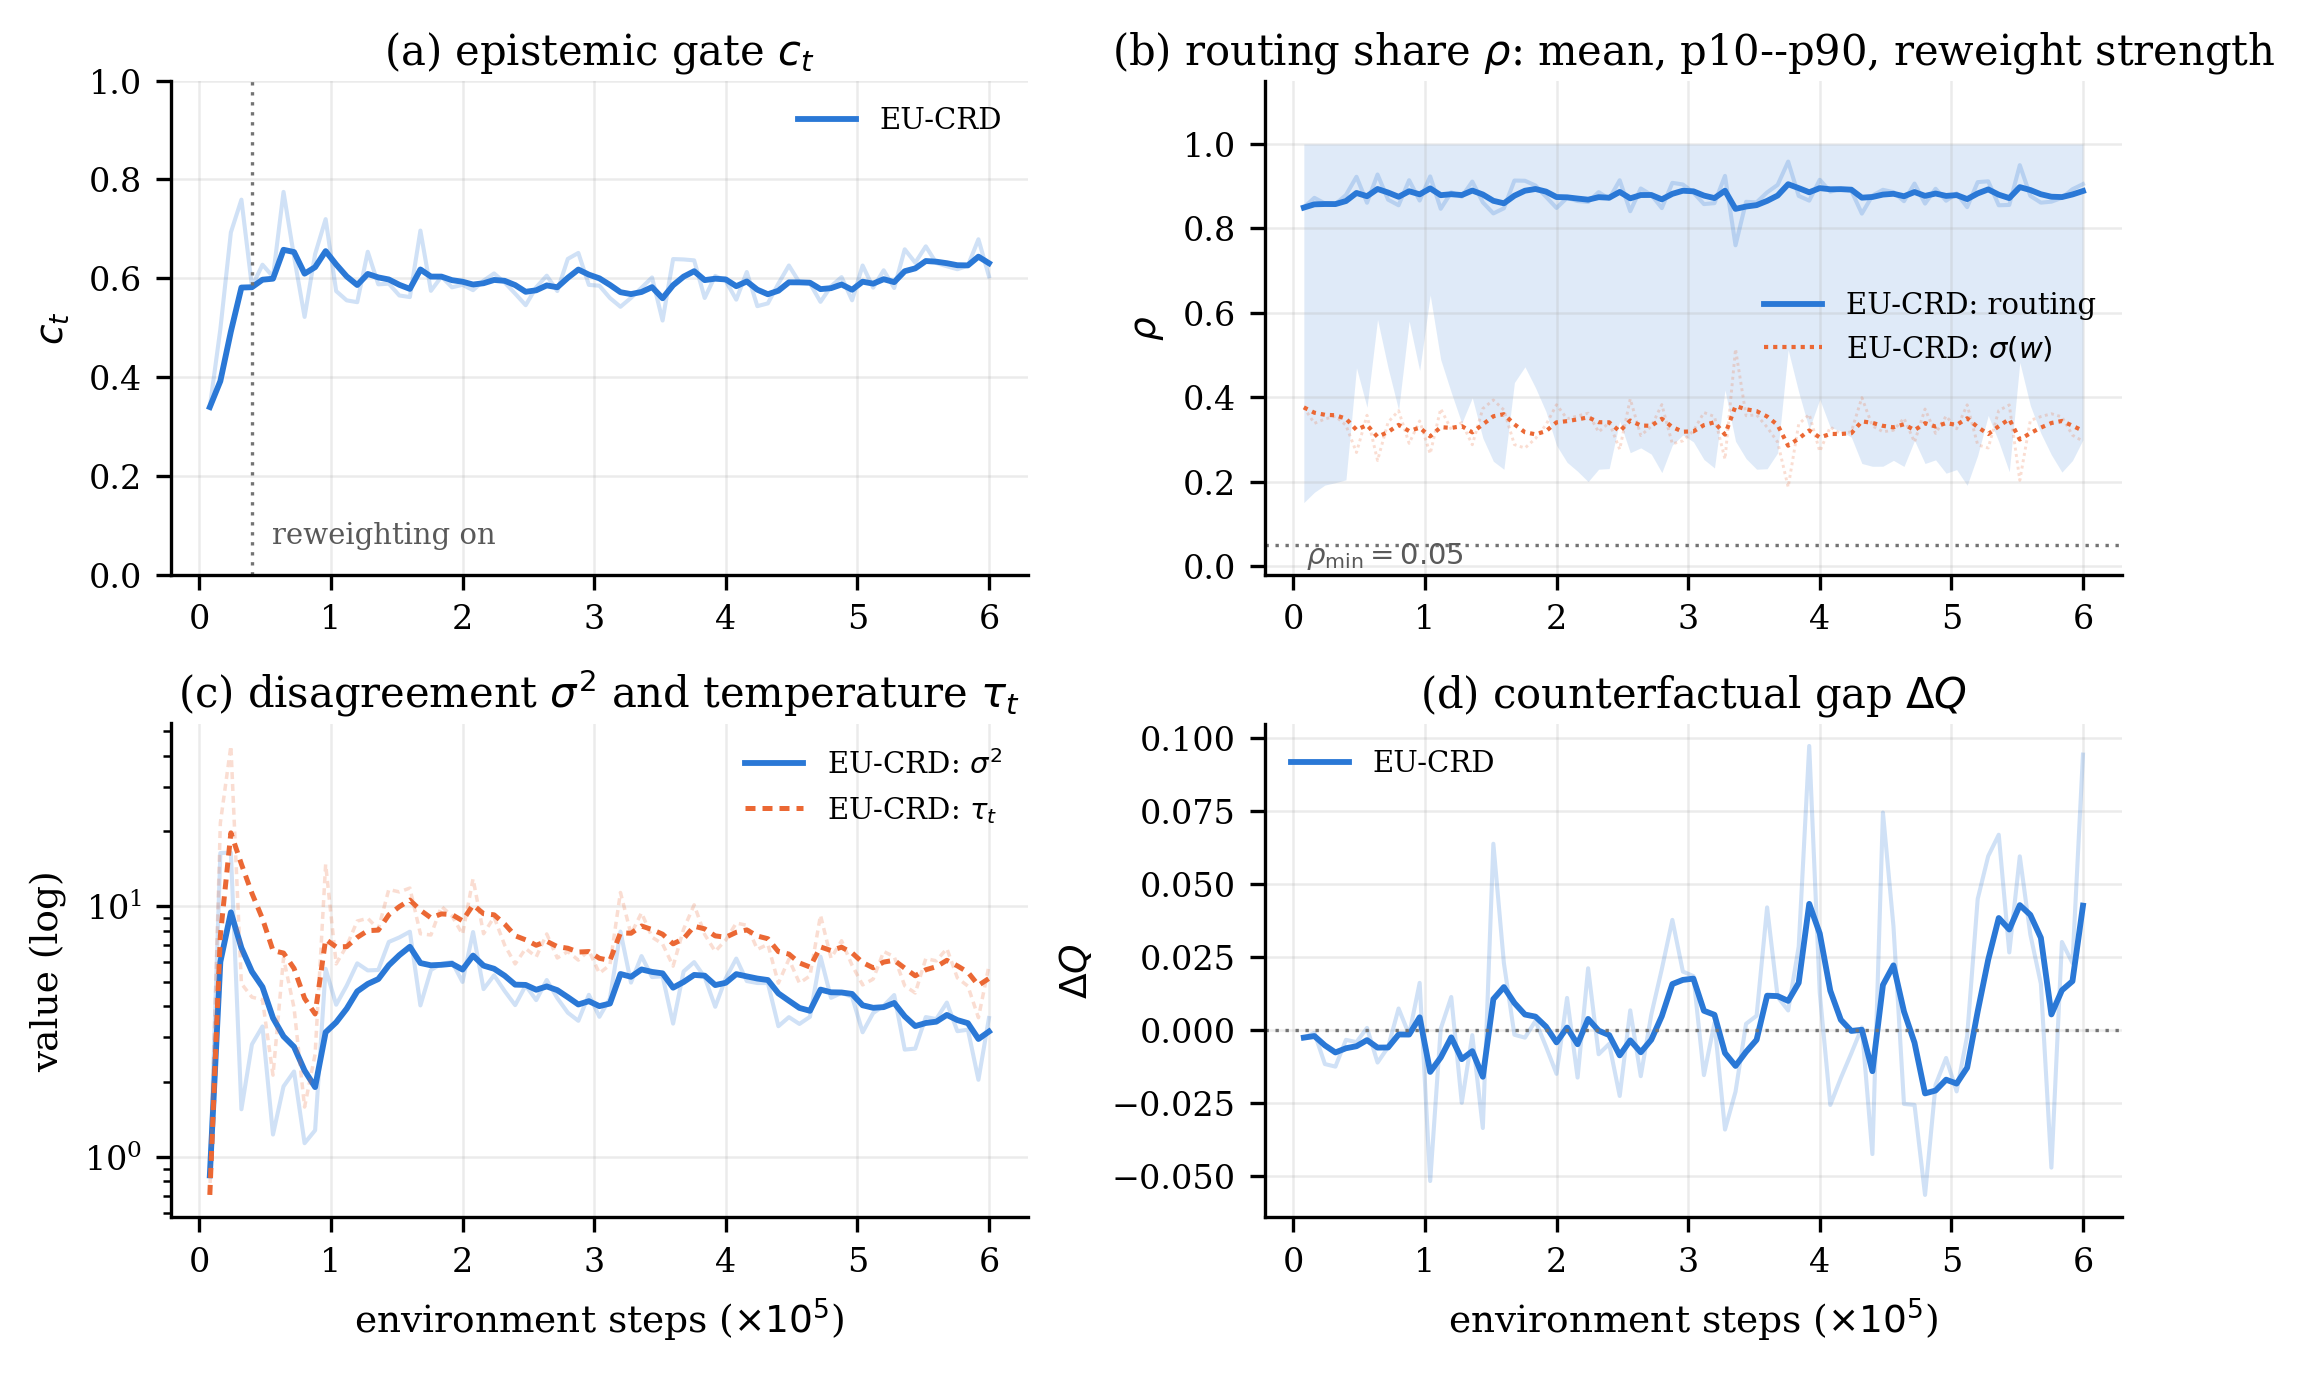
\includegraphics[width=1\linewidth]{./figs/crd_mechanism.png}
    \caption{EU-CRD training diagnostics on clean forecasts. The gate $c_t$ stays mid-range, so both credit sources contribute throughout. The routing share has a stable batch mean near $0.87$ but a wide within-batch spread ($p_{10}$--$p_{90}$ covering $0.2$ to $1.0$, reweight strength $\sigma(w)\approx0.33$). Credit is actively redistributed across transitions, not uniformly scaled. The temperature tracks the running disagreement, and the counterfactual gap stays centred near zero.}
    \label{fig:mechanism}
\end{figure}

Figure~\ref{fig:mechanism} reports the EU-CRD training diagnostics on clean forecasts, referenced from Section~\ref{sec:experiments}.

\section{Component Ablation}
\label{app:ablation}

Table~\ref{tab:ablation} reports the two component ablations against the configuration they are derived from. Each variant differs from the base in exactly one configuration key, the base arm is evaluated through the same protocol as the variants, and no cell is compared across training campaigns.

\begin{table}[ht]
\caption{Component ablation, carbon per completed work (deterministic decoding). Medians over two seeds. Each seed contributes the checkpoint with the lowest clean carbon among those completing $\geq$99.5\% on clean forecasts, the rule used in Table~\ref{tab:main}. $^{\dagger}$: at least one seed below the completion contract, carbon deflated by dropped work.
The last row is not a separate run. Disabling the decomposition leaves the matched Vanilla arm of Table~\ref{tab:main}, which differs from the full method in one configuration key, so the ladder ends where the main comparison begins and the two tables share that arm.}
\label{tab:ablation}
\centering
\small
\begin{tabular*}{\linewidth}{@{\extracolsep{\fill}}lccc@{}}
\toprule
Arm & Clean & Blend & Shuffle \\
\midrule
Base (full method)       & 0.189 & 0.186 & \textbf{0.227} \\
Gate open, $c_t\equiv1$  & 0.184 & 0.188 & 0.279$^{\dagger}$ \\
No advantage reweighting & 0.174 & 0.185 & 0.213 \\
\midrule
Decomposition off, $=$ Vanilla PPO & \ResVanClean{} & \ResVanBlend{} & \ResVanShuffle{} \\
\bottomrule
\end{tabular*}
\end{table}

The ladder ends at the matched Vanilla arm, so the ablation and the main comparison measure the same distance from two directions.

The gate carries the containment. Opening it costs nothing on clean forecasts and 23\% on shuffled ones, and the effect reproduces on both seeds separately (0.283 and 0.275 against 0.205 and 0.248). The gate-open arm is also the only one that drops work under shuffle, 99.46\% and 99.42\% against 100\% elsewhere, so its carbon is measured on a slightly smaller workload and the true gap is wider than the table shows.

The reweighting is not separately resolvable at this sample size. Removing it moves shuffle carbon from 0.227 to 0.213, within the 10 to 13\% checkpoint spread of this testbed at two seeds and one episode per cell. The ablation therefore locates the containment in the epistemic gate and leaves the marginal contribution of the reweighting open, which is the resolution this design affords.


\section{Runtime Auditor Details}
\label{app:auditor}

The auditor of Section~\ref{sec:auditor} uses the class defaults throughout, with gate threshold $\theta{=}0.2$ on the correlation averaged over green-bearing datacentres, per-datacentre repair threshold $-0.5$, window $W{=}600$ decisions, and a warmup of 120 samples during which the auditor trusts by default. At the one-second control interval these are 600 and 120 simulated seconds, about 8\% and 2\% of an episode, so the gate can engage while most of the workload is still pending. Both statistics are computed on the raw incoming forecast, never on repaired features, so a repair cannot feed back into the trust estimate and the auditor cannot oscillate. The window length trades noise against latency. A short window flags healthy forecasts on spurious dips, while a long one lets corrupted decisions accumulate before the auditor reacts. A cheaper gate could read the forecaster's own predictive uncertainty, and the argument that motivates $\chi_i$ applies against it. A coherently corrupted forecast is confidently wrong, so self-reported uncertainty stays low precisely when trust should fall. Signals over the forecast--outcome relationship do not share this blind spot.

Table~\ref{tab:auditor} reports a deployment check on one trained policy across three corruptions, run on one machine with the clean cell as the anchor, so the grid is internally consistent though its absolute values are not comparable with Table~\ref{tab:main}.

\begin{table}[ht]
\caption{Runtime auditor across three corruptions, one trained policy, three episodes per cell, deterministic decoding. Gate suppresses deferral once the cross-DC mean correlation $\chi$ falls below the threshold. Repair additionally inverts a datacentre's forecast features under strong negative correlation. Fire is the fraction of decisions the gate acted on. The inverted rows reproduce an independent ten-episode run to within 2.3\% on carbon and 0.9\,pp on completion. $^{\dagger}$: carbon deflated by dropped work, not comparable.}
\label{tab:auditor}
\centering
\small
\begin{tabular*}{\linewidth}{@{\extracolsep{\fill}}llcccc@{}}
\toprule
Forecast & Auditor & $\chi$ & Fire (\%) & Carbon & Completion (\%) \\
\midrule
clean (anchor) & off    & $+0.71$ & 0.0  & 0.185 & 99.9 \\
\addlinespace
inverted       & off    & $-0.71$ & 0.0  & 0.126$^{\dagger}$ & 79.1 \\
inverted       & gate   & $-0.71$ & 99.4 & 0.203 & 96.4 \\
inverted       & repair & $-0.71$ & 99.4 & \textbf{0.178} & \textbf{99.9} \\
\addlinespace
neutralised    & off    & $\phantom{+}0.00$ & 0.0  & 0.131$^{\dagger}$ & 95.9 \\
neutralised    & gate   & $\phantom{+}0.00$ & 99.4 & 0.182 & 98.8 \\
\addlinespace
reassigned     & off               & $+0.23$ & 0.0  & 0.226 & 100.0 \\
reassigned     & gate ($\theta{=}0.2$) & $+0.23$ & 14.9 & 0.219 & 100.0 \\
reassigned     & gate (calibrated) & $+0.23$ & 99.4 & 0.214 & 100.0 \\
\bottomrule
\end{tabular*}
\end{table}

Four readings follow. First, the forecast is load-bearing at deployment. Inverting it costs twenty percentage points of completion on a policy that otherwise finishes the entire workload. Second, the carbon of the unaudited inverted and neutralised cells is below the anchor only because a fifth and a twentieth of the work is never done, the selection effect Section~\ref{sec:experiments} guards against, so neither cell carries a carbon claim. Third, on the inversion the auditor works and repair works better than gating alone. Suppressing deferral recovers most of the completion at a ten percent carbon premium, whereas inverting the flagged features restores the clean operating point on both axes at once, 0.178 against 0.185 clean and 99.9\% against 99.9\%. The chain from corruption to detection to restoration closes on a single policy, which is the property Section~\ref{sec:auditor} claims.

Fourth, the audit has two blind spots, one of which calibration closes. Under a reassigned forecast $\chi$ settles at $+0.23$, above the class default $\theta{=}0.2$, so the gate acts on only 14.9\% of decisions and the corruption passes essentially unchallenged. The statistic is not at fault, since $+0.23$ is far below the $+0.71$ a healthy forecast produces. The fixed threshold is what fails. Re-registering the threshold relative to the clean operating point, at half of the $\chi$ the same policy shows on clean forecasts, raises the fire rate to 99.4\% and holds completion at 100\%, at a cost of firing on 0.5\% of clean decisions. The carbon differences among the three reassigned cells fall within the few-percent run-to-run spread of a three-episode cell and no carbon claim is made on them. What the calibration demonstrably fixes is detection, not saving. The residual limitation is structural. Blending a forecast towards a constant is an affine shrink, and correlation is invariant to affine transformation, so $\chi$ stays near its clean value under partial neutralisation and collapses only when the last of the variance is gone. A trust statistic built on correlation therefore sees coherent lies and complete silence, but not gradual loss of information, and detecting that case needs a scale-sensitive statistic alongside it.

The matched EU-CRD checkpoint is omitted from this table. Its training-time completion fell from 100\% to 78\% over the final third of training and its clean deployment completion is 16.7\%, so its cells measure a diverged policy rather than the method, and no robustness reading can be taken from them.

\section{Deployment Overhead}
\label{app:overhead}

\begin{table}[t]
\caption{Deployment overhead. Global and local decision latency measure the time to route one batch or drain one queue, ratios are relative to Round-Robin, and Wall is the end-to-end wall clock of one full evaluation episode (not measured for the two single-seed risk baselines). All learned methods share the GTrXL backbone and therefore incur the same inference cost by construction, so the differences between them fall entirely within training.}
\label{tab:overhead}
\centering
\small
\begin{tabular*}{\linewidth}{@{\extracolsep{\fill}}lccccc@{}}
\toprule
Method & Global dec. & Local dec. & Peak RSS & Wall & Latency \\
       & mean/p99 ($\mu$s) & mean/p99 ($\mu$s) & (MB) & (s) & vs.\ RR \\
\midrule
Round-Robin      & 29/34      & 3/14    & 1066 & 273 & 1.0$\times$ \\
Vanilla PPO      & 2044/20165 & 467/600 & 1323 & 318 & 70.4$\times$ \\
Risk-sensitive   & 2089/21113 & 467/600 & 1323 & --  & 71.9$\times$ \\
CVaR-PPO         & 2080/20977 & 466/603 & 1324 & --  & 71.6$\times$ \\
\textbf{EU-CRD}  & 2069/20967 & 475/611 & 1329 & 319 & 71.2$\times$ \\
\bottomrule
\end{tabular*}
\end{table}

Two points stand out. First, the learned methods are indistinguishable at deployment. Every reinforcement learning policy routes a batch in about 2.1\,ms and drains a queue in about 0.47\,ms, within a few percent of one another and of Vanilla PPO, because they share one backbone while the counterfactual decomposition, the critic ensemble, and the responsibility reweighting in EU-CRD all act on the training signal alone and leave the deployed policy a plain forward pass. The runtime auditor adds only a rolling correlation per datacentre, which is negligible against the network evaluation, and inference uses no GPU, so the scheduler runs on commodity hardware. EU-CRD is therefore no more expensive to deploy than the Vanilla PPO that it improves upon.

Second, the learned policies cost about $70\times$ a trivial heuristic per decision, yet the absolute figure of roughly two milliseconds to route a batch is immaterial on the scheduling timescale, where a control interval spans seconds of simulated time. Training is where the ensemble is paid for. In profiling runs the EU-CRD learner update costs roughly a quarter more than Vanilla's per iteration, while the end-to-end wall clock differs by well under one percent (Table~\ref{tab:overhead}) because the environment simulation, not the learner, dominates it. The decomposition thus buys its robustness during training and provides it at no cost during deployment.

\section{Reward Design}
\label{app:reward}

The two reward channels mirror the hierarchical division of Section~\ref{sec:mdp}. The global reward carries the carbon objective and is additively decomposable over the routing slots,
\begin{equation}
r^{G}_t=\sum_{i\in\text{routed}}
\big(-w_c\,\hat{m}_i+w_p\,\hat{P}_i\big)
-\sum_{i\in\text{deferred}}\big(c_0+w_u\,\nu_i\big),
\label{eq:reward}
\end{equation}
where $\hat{m}_i$ is the normalised marginal carbon of placing job $i$ at its chosen DC given the current green headroom, and $\hat{P}_i=\exp(-k\,o_i)$ a congestion proxy for on-time completion with $o_i=\max\{0,(Q_d+\mathrm{pe}_i-a_d)/\Gamma_d\}$ the fraction by which admitting job $i$ (of PE demand $\mathrm{pe}_i$) would push the chosen DC $d$ past its available capacity $a_d$, relative to total capacity $\Gamma_d$, and $k$ setting the sharpness. The last term uses $\nu_i=\min\{1,\max\{0,\, 1-(d_i-t)/W_u\}\}$, an urgency ramp that grows as the deadline $d_i$ approaches. Deferral is thus never free. The base cost $c_0$ prices the option of waiting, and the urgency term makes procrastination on near-deadline work expensive. The local reward is a standard quality-of-service signal with no carbon term,
\begin{equation}
\begin{split}
r^{L}_t={} & \lambda_1\log(1{+}n_t)-\lambda_2\log(1{+}\bar{W}_t) \\
& -\lambda_3\,\operatorname{std}_v\rho_{v,t}-\lambda_4\frac{Q_t}{R_t}
-\lambda_5\,\mathds{1}[\text{invalid}],
\end{split}
\label{eq:localreward}
\end{equation}
which rewards the $n_t$ completions in the step and penalises the mean wait $\bar{W}_t$ of finished jobs, the imbalance $\operatorname{std}_v\rho_{v,t}$ of utilisation across active VMs, the backlog ratio $Q_t/R_t$ of queued to received jobs, and invalid actions. Carbon and the forecast both enter only through $r^{G}_t$, so the local reward is forecast-independent. The coefficients, identical across all methods, are $w_c{=}1.0$, $w_p{=}2.0$, $k{=}6.0$, $c_0{=}0.5$, $w_u{=}2.0$, $W_u{=}3{,}600$\,s (with $\hat m_i$ normalised by 0.05\,kg), and $\lambda_{1\ldots5}=0.3,\,0.05,\,0.02,\,0.05,\,0.2$. The decomposition of Section~\ref{sec:crd} dissects the credit carried by $r^{G}_t$ alone. The local channel passes through untouched.

The reward-level fallback of Eq.~\ref{eq:blend} is the green-fit contrast of Eq.~\ref{eq:deltar}, with $\alpha{=}1$. It is evaluated slot by slot on the routing batch. Each slot contributes the green ratio of the datacentre the router chose minus the green ratio of the datacentre the reference action would have chosen, DEFER slots contribute zero, and the per-transition value is the mean over slots. Both terms read the observation the router already saw, so the reference routing never needs to be executed, and the contrast keeps the chosen-minus-reference semantics of $\Delta Q$. Orientation matters here. A positive $\Delta r$ means the router placed work on greener sites than the reference, which is the sign convention $\Delta Q$ carries, so the soft blend mixes two estimators of the same quantity rather than two different ones. An earlier version of this fallback measured load dispersion instead. Under the per-action carbon reward used here, load balance is not a term in the reward at all, so that proxy tracked a quantity the objective does not contain and could disagree with $\Delta Q$ in sign. The green-fit form replaces it.




\end{document}
